\chapter{Analysis of Results}
In this chapter, we are going to analyze the evolution and final results of the two models (see chapter \ref{methods:both_models}), trained on the OpenSubtitles and Reddit corpus, under several different aspects. This includes the analysis of the learning process throughout the training. Then we are going to analyse the language model of the trained models and try to find a correlation between the language model in the training dataset and the language model the trained models produce.\todo{Two times model is ugly!} In the end, we are going to focus on how well the model understands and percepts them, combined with an analysis

\begin{enumerate}[noitemsep]
	\item \textbf{Quantitive}: This part focuses on evaluating metrics and other measurements. We are going to look into the metrics at train time, a similarity analysis using Sent2Vec and an analysis of the produced language models by using n-gram collocations.\todo{Not correct: What are we going to do with ngrams?}
	\item \textbf{Qualitative}: This part focuses on the quality of the language produced by the models. This includes a comparison between our models and \emph{CleverBot}\footnote{http://www.cleverbot.com/} and the development of the language model of the models throughout the training time.
	\item \textbf{Miscellaneous}: This part focuses on theoretical analysis, such as analyzing the internal embeddings for the input sequence or if and how the models are using the soft-attention mechanism in their favor.
\end{enumerate}

The analysis is done in the order listed above, that means we start by analysing the quantitive measures
\blindtext

* Attention
* Learning process
* Generated outputs over time
* Generation at the end and comparison with cleverbot and paper
* Generated outputs at the end and related ngram analysis
* Generated embeddings for input sentences
* Sent2Vec analysis

\section{How Did The Training Go?}
First, let us start by analysing the evolution of the models with regard to the available performance metrics throughout the time span of the training. Below, in Figures~\ref{results:learning_process:metrics:opensubtitles} and~\ref{results:learning_process:metrics:reddit}, one can see the development of the loss and perplexity on the training sets for the two different models. What is eye-catching when comparing the two is that the OpenSubtitles seems to have much more variance in its performance on the validation set as opposed to the Reddit model. This probably comes from the fact that the OpenSubtitles datasets are much more noisey than the one of the Reddit model, as \cite{Vinyals:2015} also already noticed. This has to do with the fact, that we do not have any information about turn taking, which means it is certainly possible that consecutive utterances may be uttered by the same person even though we treat it if it were two persons. Also, there is the problematic with the time lags between utterances as analysed in Chapter~\ref{data:opensubtitles:time_lag_analysis}. In contrast, with the Reddit dataset, we always know who uttered a comment and hence can build a dataset which ensures that the dialogs make sense from a structural perspective.

\begin{figure}[H]
	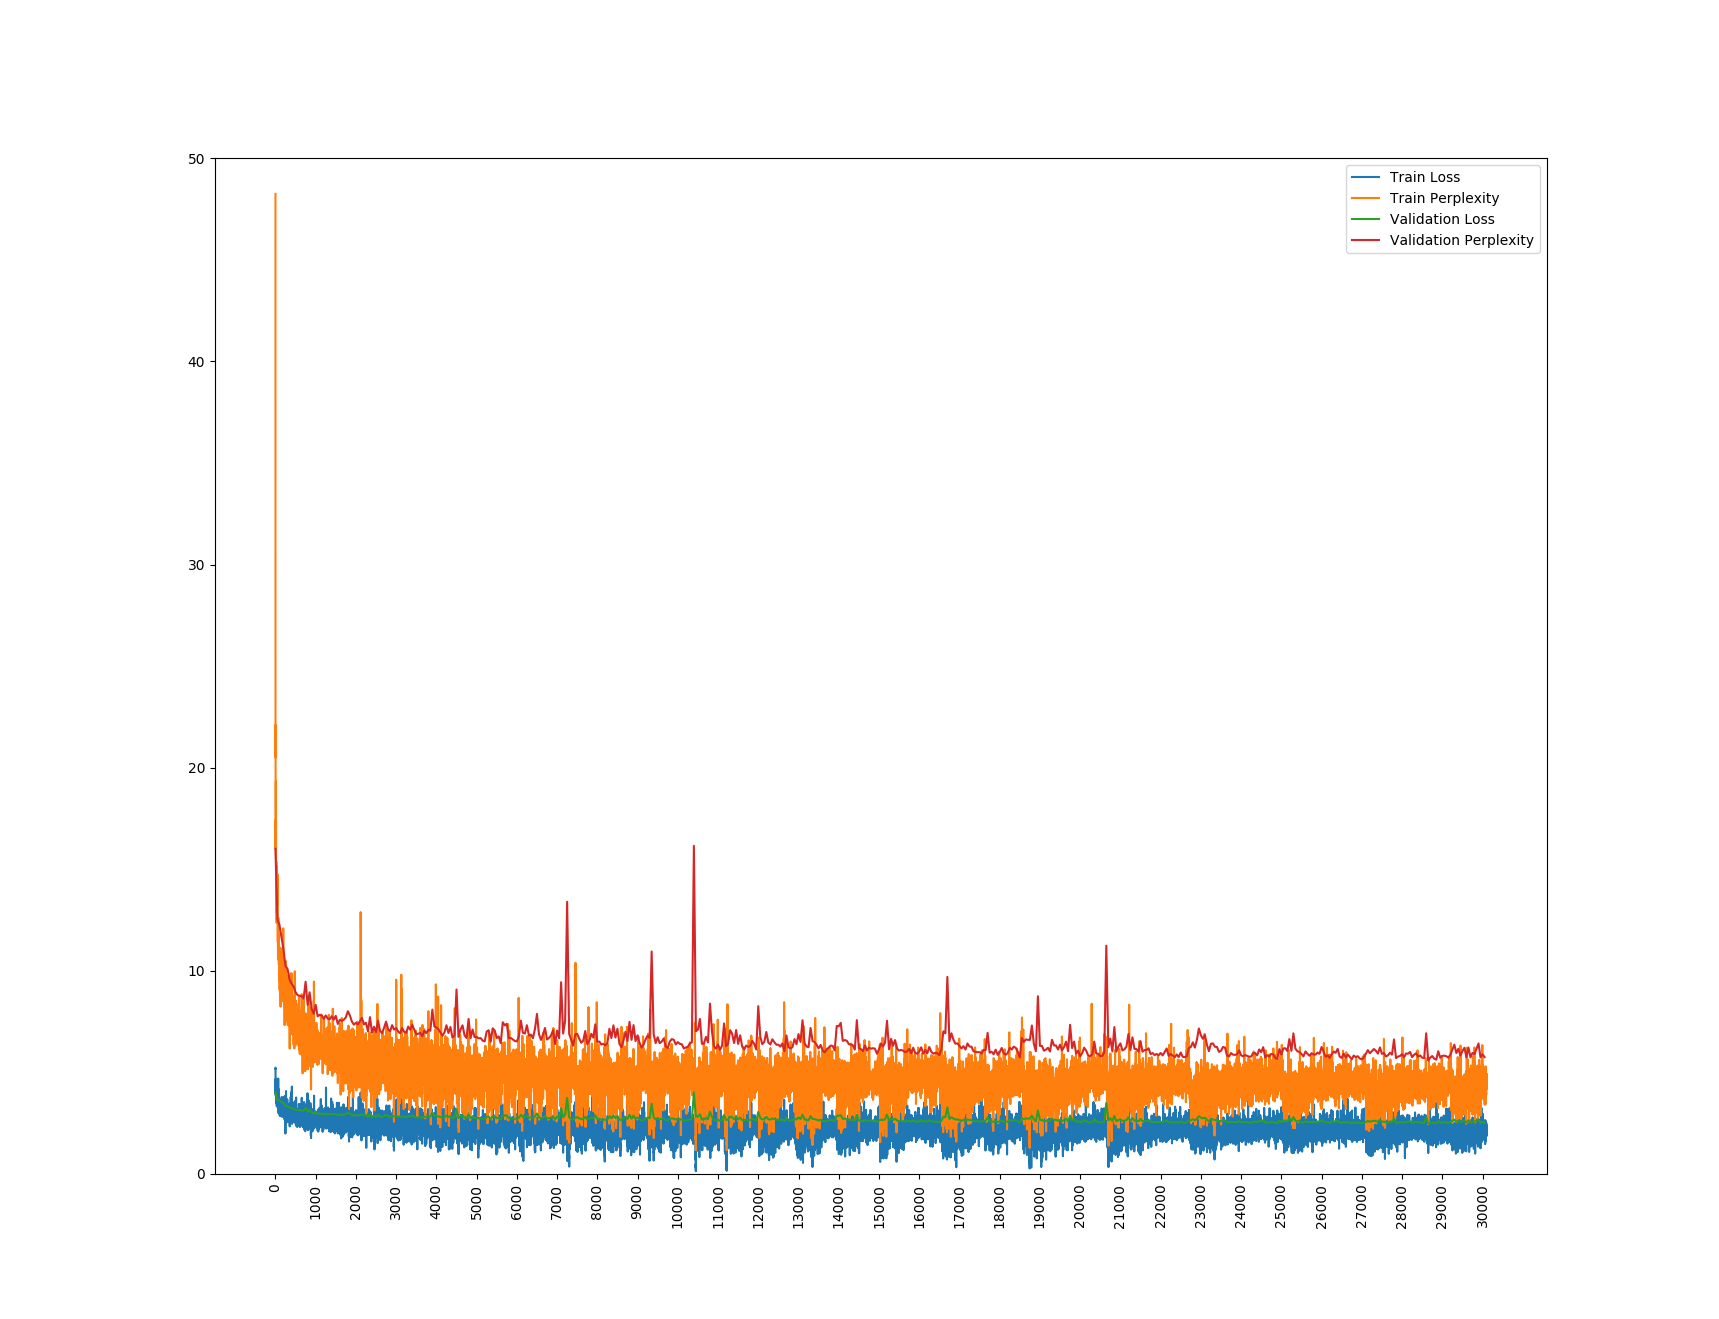
\includegraphics[width=\linewidth]{img/plots/opensubtitles_not_reversed/train_metrics.png}
	\caption{Development of the loss and perplexity on the training and validation set throughout the training of the OpenSubtitles model.}
	\label{results:learning_process:metrics:opensubtitles}
\end{figure}

The interesting part about the learning process of the Reddit model are the ``dips'' in the validation perplexity and hence in the loss on the validation dataset, even though there they are not as easily noticeable.\todo{Write more!}

\begin{figure}[H]
	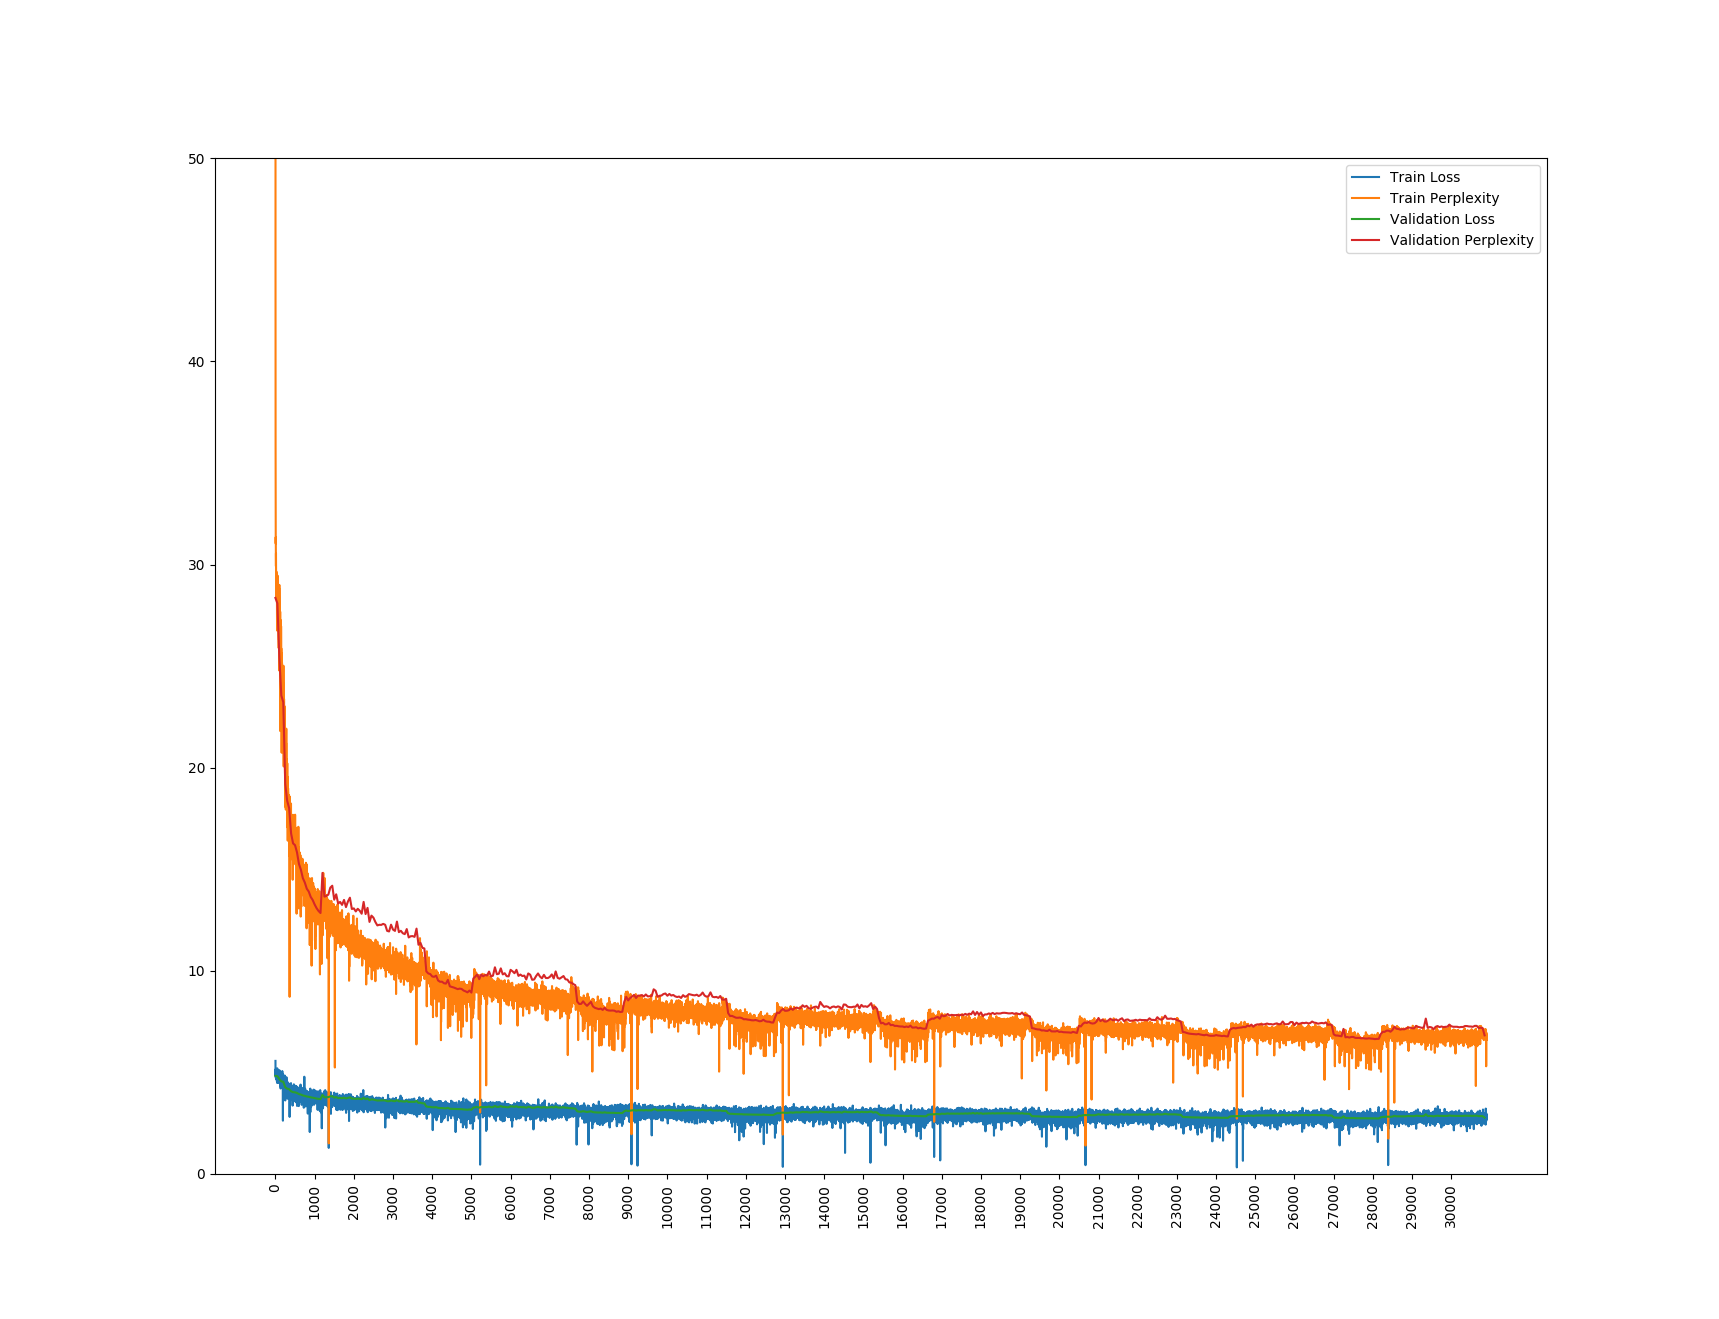
\includegraphics[width=\linewidth]{img/plots/reddit/train_metrics.png}
	\caption{Development of the loss and perplexity on the training and validation set throughout the training of the Reddit model.}
	\label{results:learning_process:metrics:reddit}
\end{figure}

When looking at the metrics from the training, the results seem fine.

\section{How is the Performance when Evaluating the Models?}
After we have seen that the training process looks fine, we are going to asses the performance of these models on our test datasets. Here we use the same metrics as within the training, namely the loss and perplexity values. We have evaluated each model on the respective test dataset for each checkpoint we have created while training (see Chapter~\ref{methods}). The resulting values are visualized in the Figures~\ref{result:test_performance:opensubtitles} and~\ref{result:test_performance:reddit}.

\begin{figure}[H]
	\minipage{0.5\textwidth}
	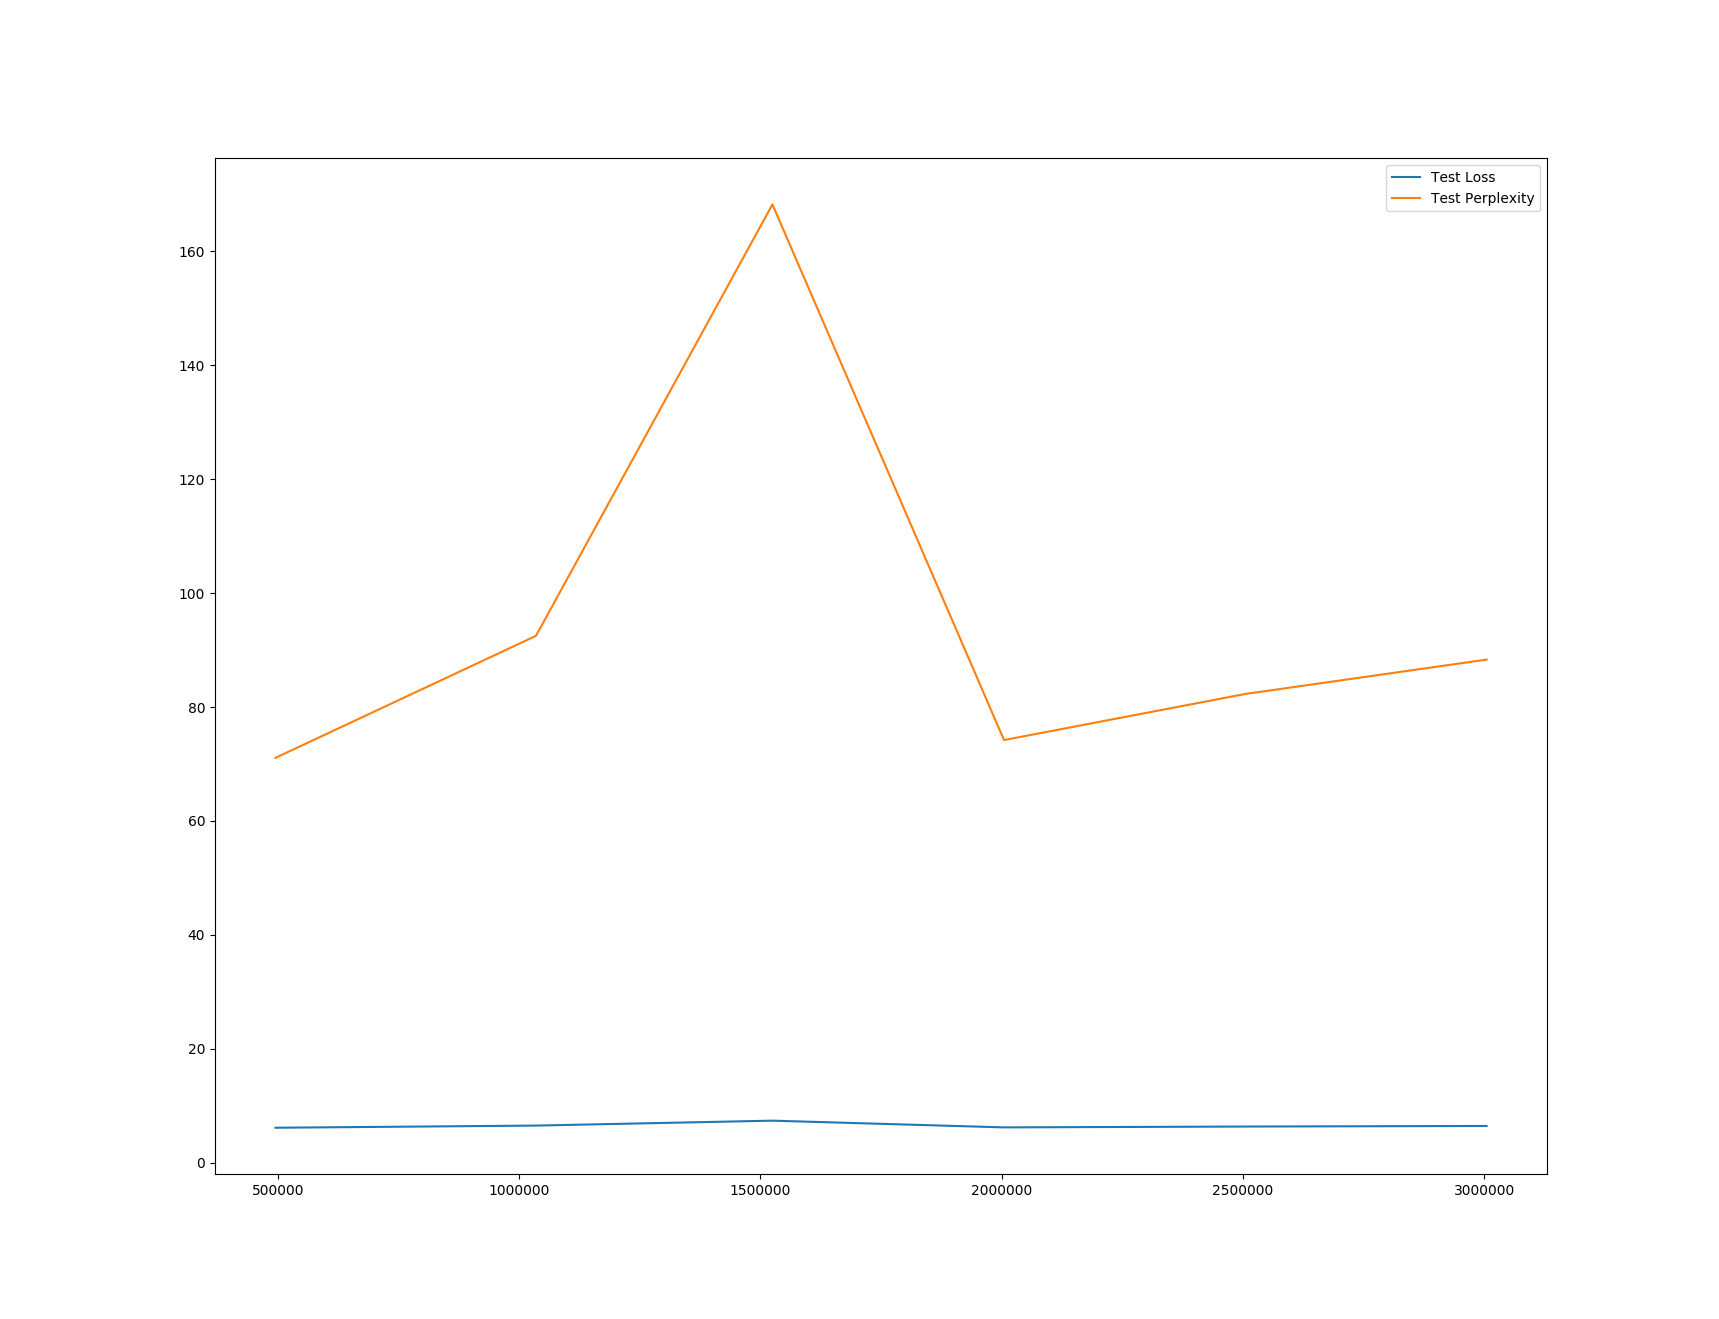
\includegraphics[width=\linewidth]{img/plots/opensubtitles_not_reversed/test_metrics_both.png}
	\centering
	\small
	\text{The loss and perplexity.}
	\endminipage\hfill
	\minipage{0.5\textwidth}
	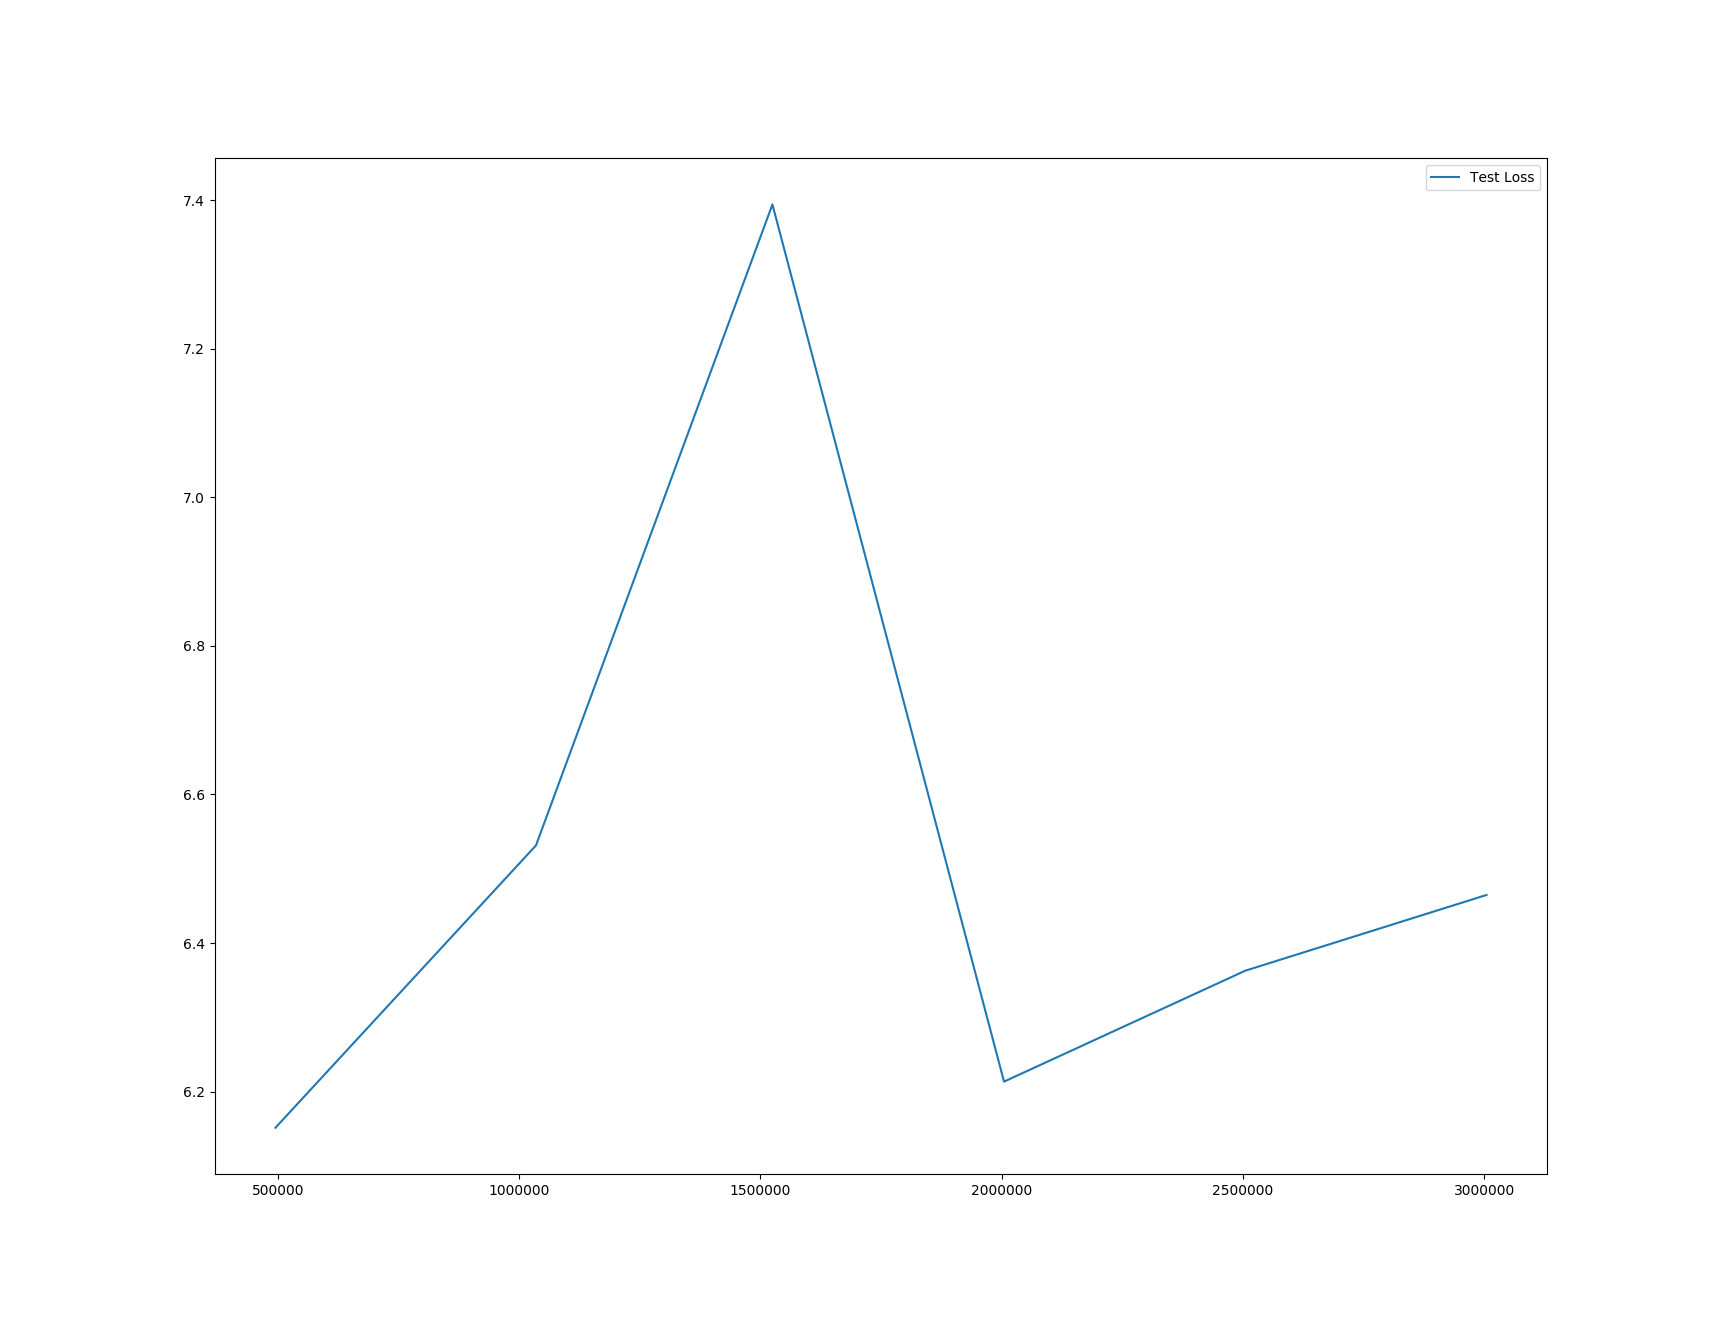
\includegraphics[width=\linewidth]{img/plots/opensubtitles_not_reversed/test_metrics_loss.png}
	\centering
	\small
	\text{Only the loss.}
	\endminipage\hfill
	\caption{The loss and perplexity by running the six different snapshots against the test dataset using the OpenSubtitles model.}
	\label{result:test_performance:opensubtitles}
\end{figure}

\begin{figure}[H]
	\minipage{0.5\textwidth}
	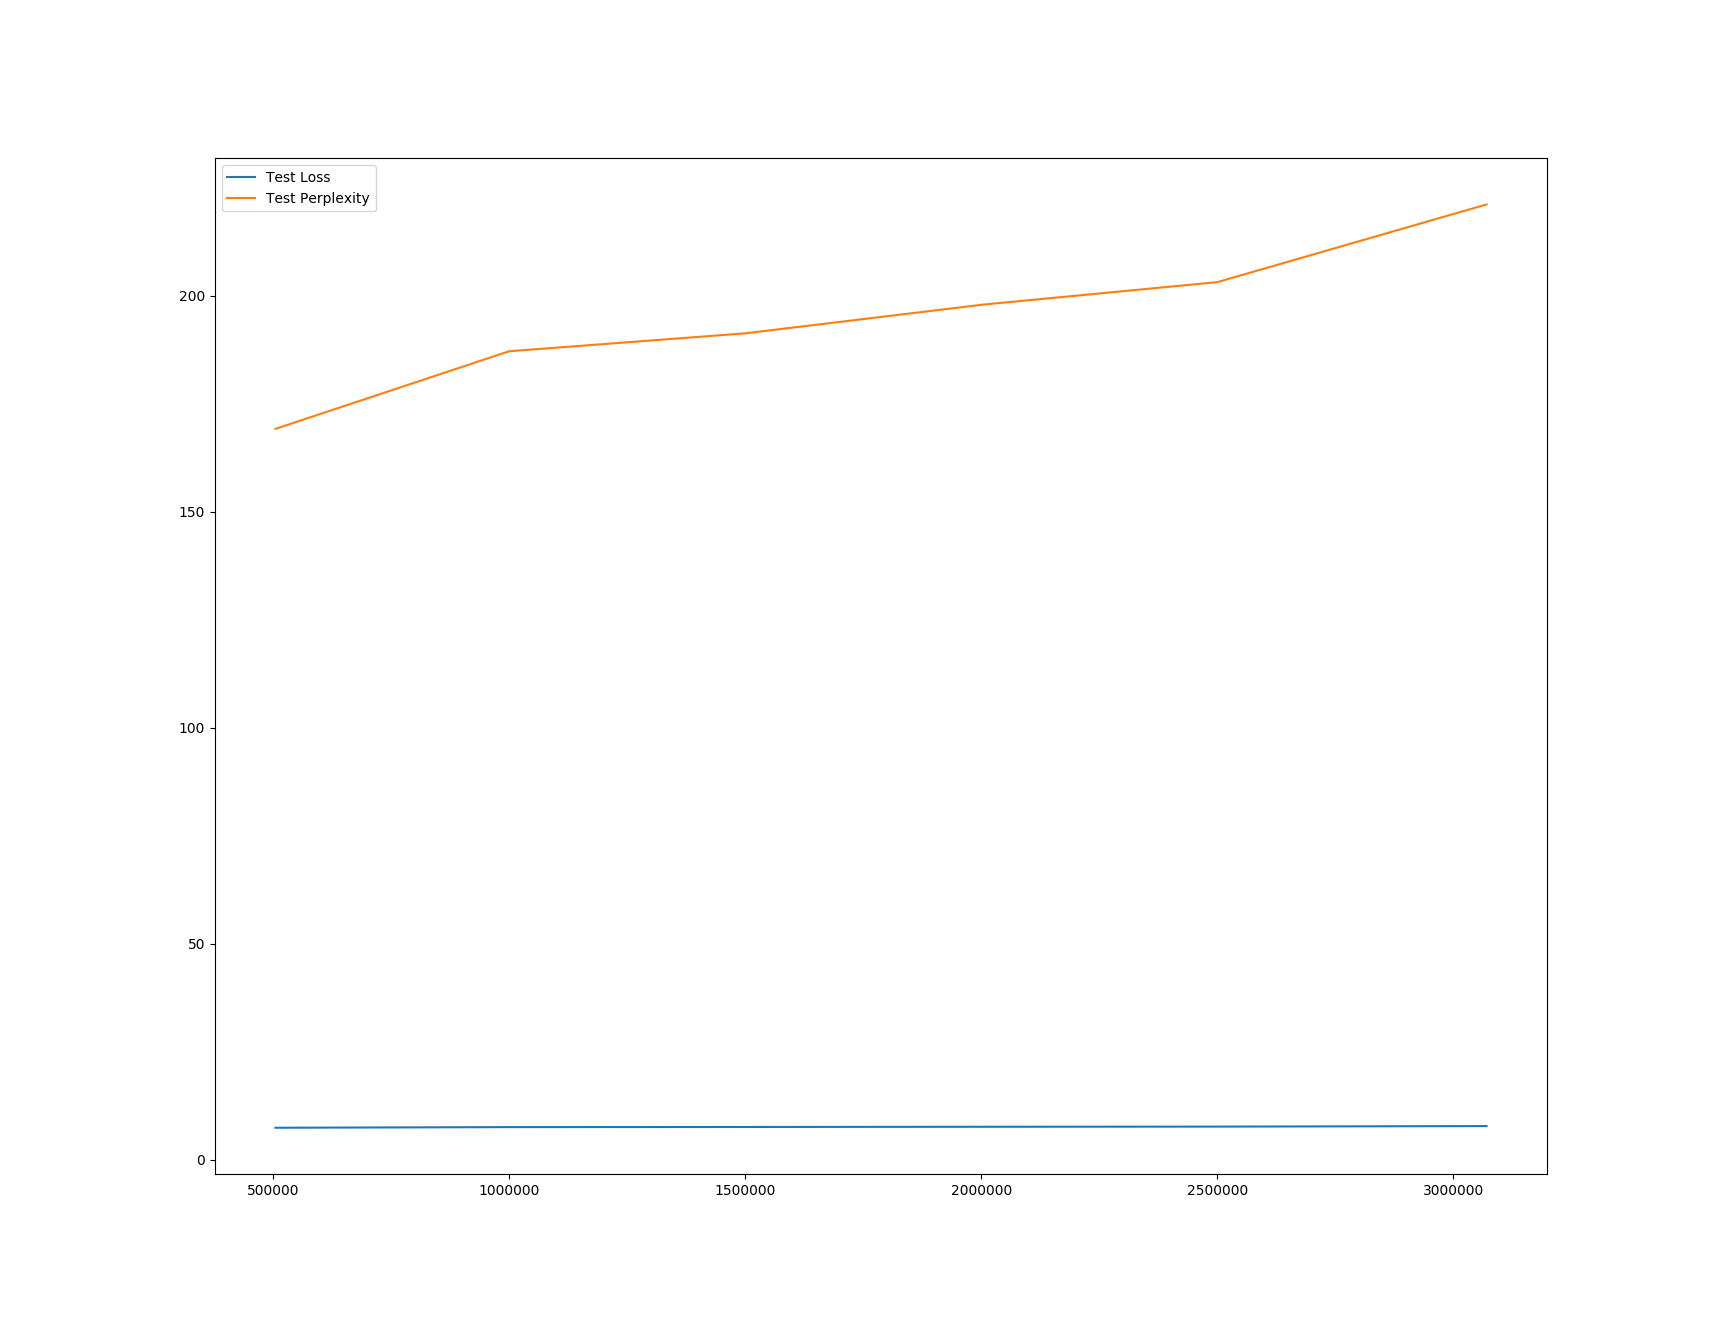
\includegraphics[width=\linewidth]{img/plots/reddit/test_metrics_both.png}
	\centering
	\small
	\text{The loss and perplexity.}
	\endminipage\hfill
	\minipage{0.5\textwidth}
	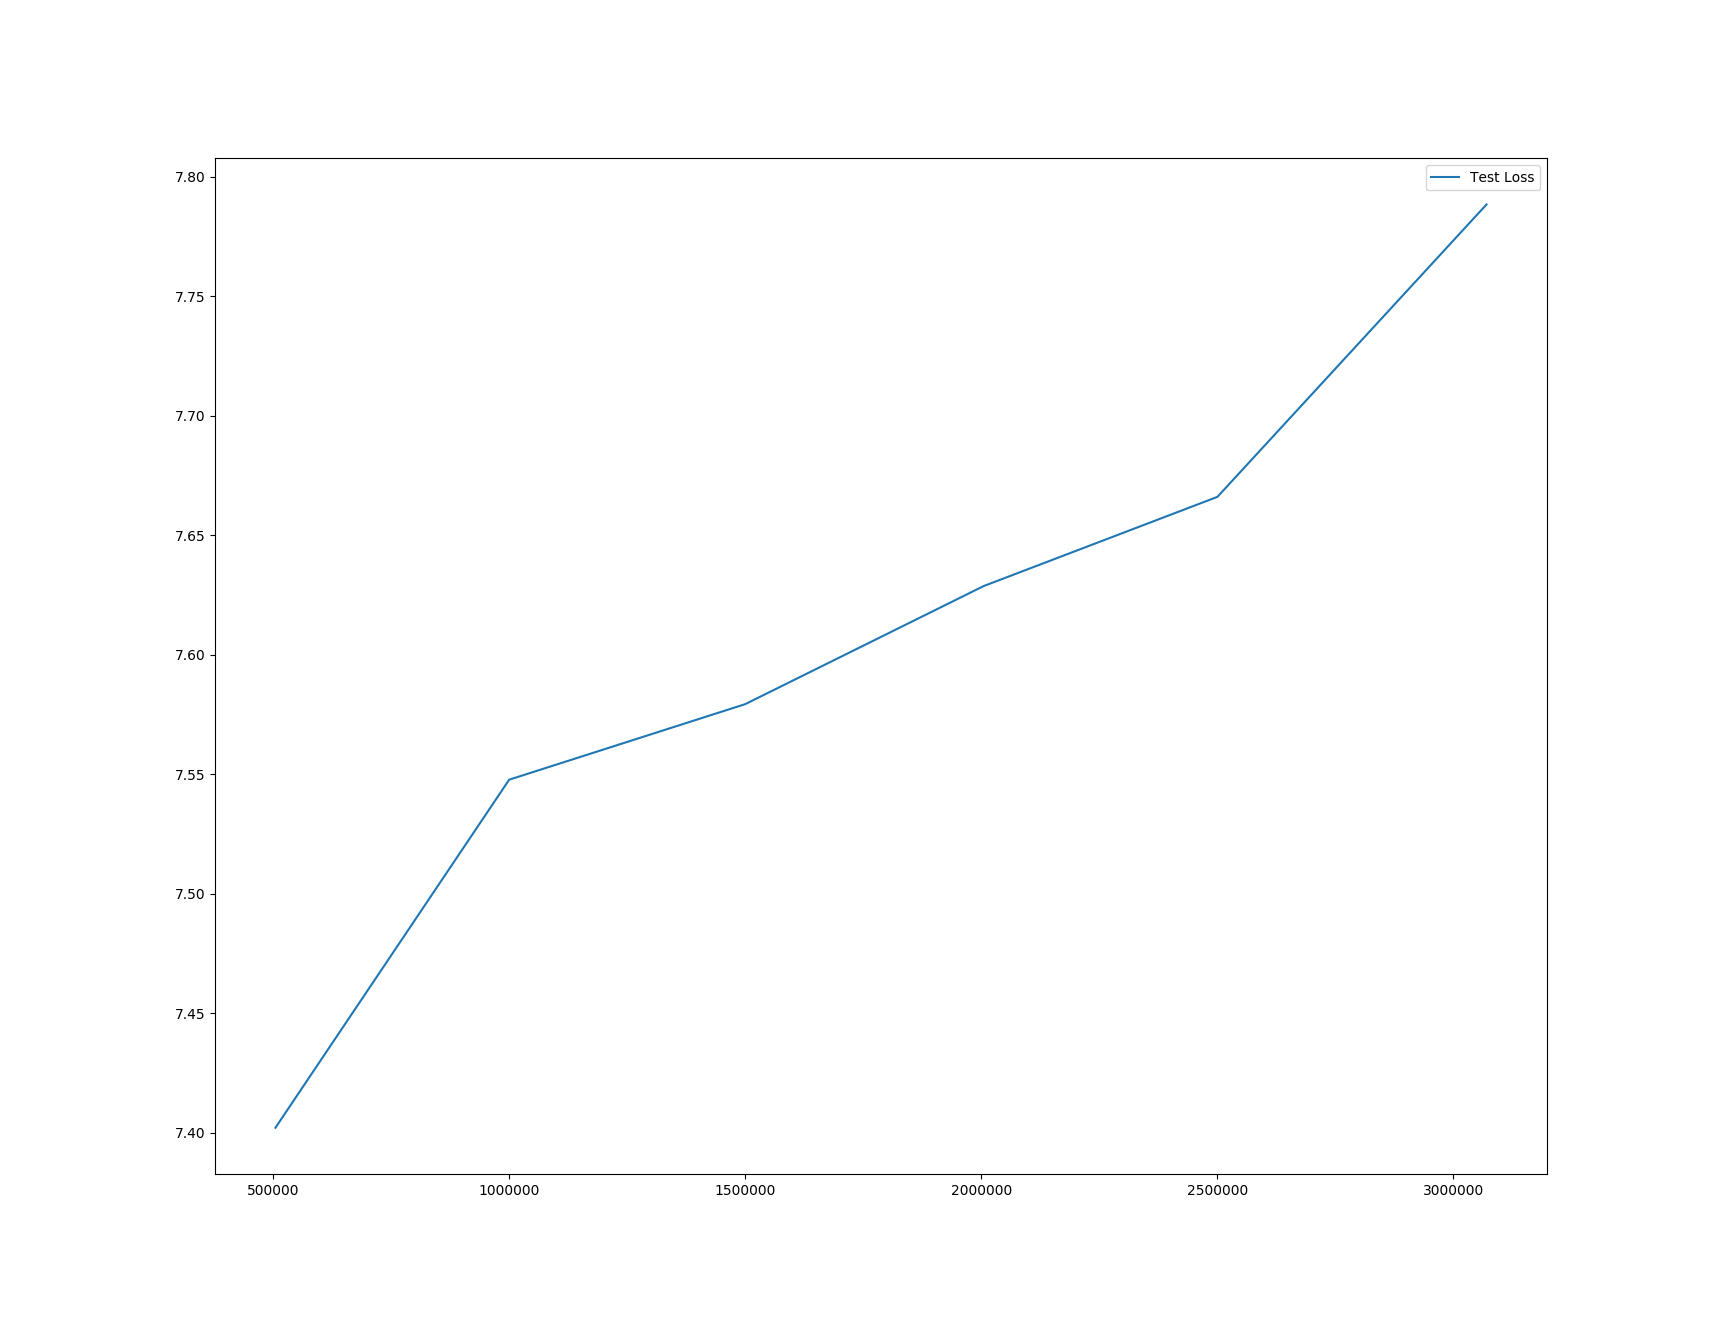
\includegraphics[width=\linewidth]{img/plots/reddit/test_metrics_loss.png}
	\centering
	\small
	\text{Only the loss.}
	\endminipage\hfill
	\caption{The loss and perplexity by running the six different snapshots against the test dataset using the Reddit model.}
	\label{result:test_performance:reddit}
\end{figure}

Apparently, the results on the test set are quite the opposite of the results from the training process. We did not expect that, but nevertheless, we are going to analyse the problem. Our first idea was, to see, what kind of sentences the models produce on the test dataset. We did an analysis on the generated sentences and quickly noticed, that there are a few sentences, which the models predict a lot of time (see Tables~\ref{results:test_performance:opensubtitles_sample_outputs} and~\ref{results:test_performance:reddit_sample_outputs}).

\begin{table}[H]
	\centering
	\ra{1.3}
	\begin{adjustbox}{max width=\textwidth}
		\begin{tabular}{ll}
			\toprule
			Sentence & Frequency\\ \midrule
			\texttt{i m not gon na let you go} & 41853\\
			\texttt{i m not sure i can trust you} & 21263\\
			\texttt{i m not gon na say anything} & 9163\\
			\texttt{i m not gon na let that happen} & 7426\\
			\texttt{i m sorry} & 7235\\
			\texttt{you re not gon na believe this} & 7068\\
			\texttt{you re not gon na believe me} & 6878\\
			\texttt{i m not gon na hurt} you & 4829\\
			\texttt{i m not a fan} & 4468\\
			\texttt{i m not sure} & 4215\\
			\bottomrule
		\end{tabular}
	\end{adjustbox}
	\caption{Top 10 most generated sentences with respective occurence frequencies when using the last OpenSubtitles model on the test dataset.}
	\label{results:test_performance:opensubtitles_sample_outputs}
\end{table}

\begin{table}[H]
\centering
\ra{1.3}
\begin{adjustbox}{max width=\textwidth}
	\begin{tabular}{ll}
		\toprule
		Sentence & Frequency\\ \midrule
		\texttt{i m not sure if i m being sarcastic or not .} & 17486\\
		\texttt{i think it s a bit of a stretch .} & 13058\\
		\texttt{i m not sure if you re being sarcastic or not .} & 11647\\
		\texttt{i m not sure if i m a <unknown> or not .} & 8307\\
		\texttt{i m not sure if you re joking or not .} & 7932\\
		\texttt{i was thinking the same thing .} & 7579\\
		\texttt{<unknown>} & 6210\\
		\texttt{i m not sure if i m going to watch this or not .} & 4257\\
		\specialcell{\texttt{i m not sure if i m a fan of the show , but i m}\\\texttt{pretty sure that s a <unknown> .}} & 3232\\
		\texttt{i m not sure if i m going to watch it or not .} & 3079\\
		\bottomrule
	\end{tabular}
\end{adjustbox}
\caption{Top 10 most generated sentences with respective occurence frequencies when using the last Reddit model on the test dataset.}
\label{results:test_performance:reddit_sample_outputs}
\end{table}

\section{What Language Model do the Models produce?}
\blindtext

\section{Does the Model have an understanding of natural language?}
\blindtext

\section{How can we fix the detected problems?}
\blindtext

\section{Performance on Test Sets}
The models were evaluated on the test set after the training has been finished. In total, we evaluated both models on all six checkpoints and the results can be seen in the Figures~\ref{result:test_performance:opensubtitles} and~\ref{result:test_performance:reddit}. The results of the OpenSubtitles model seem to vary across the different checkpoints, with the best result having a perplexity of $71.07$ and a loss of $6.15$ and coming from the evaluation with the first checkpoint. The best result of the Reddit model is also achieved on the first checkpoint, with all other checkpoints having a worse perplexity.

This result stands in contradiction to what we have expected. Instead of 

\begin{figure}[H]
	\minipage{0.5\textwidth}
	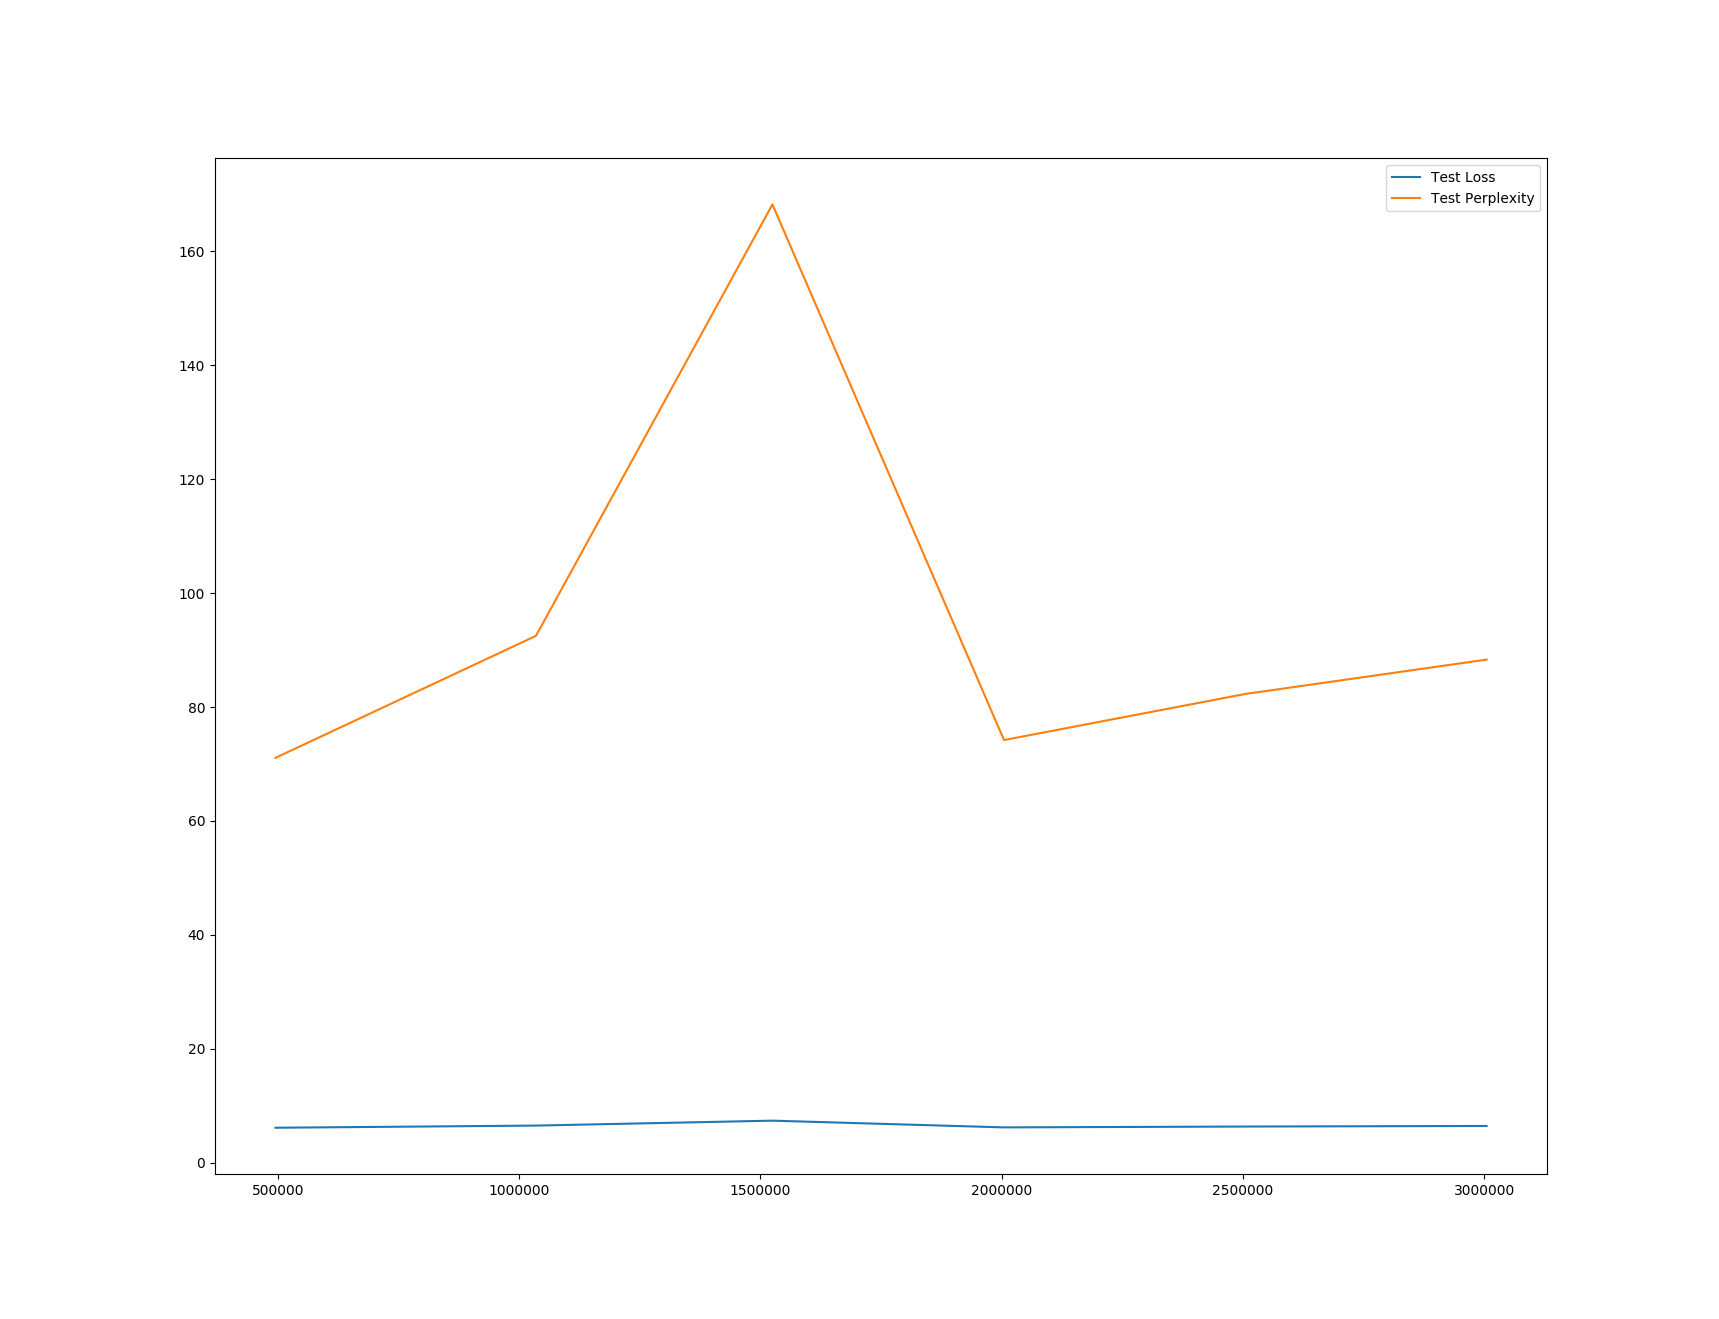
\includegraphics[width=\linewidth]{img/plots/opensubtitles_not_reversed/test_metrics_both.png}
	\centering
	\small
	\text{The loss and perplexity.}
	\endminipage\hfill
	\minipage{0.5\textwidth}
	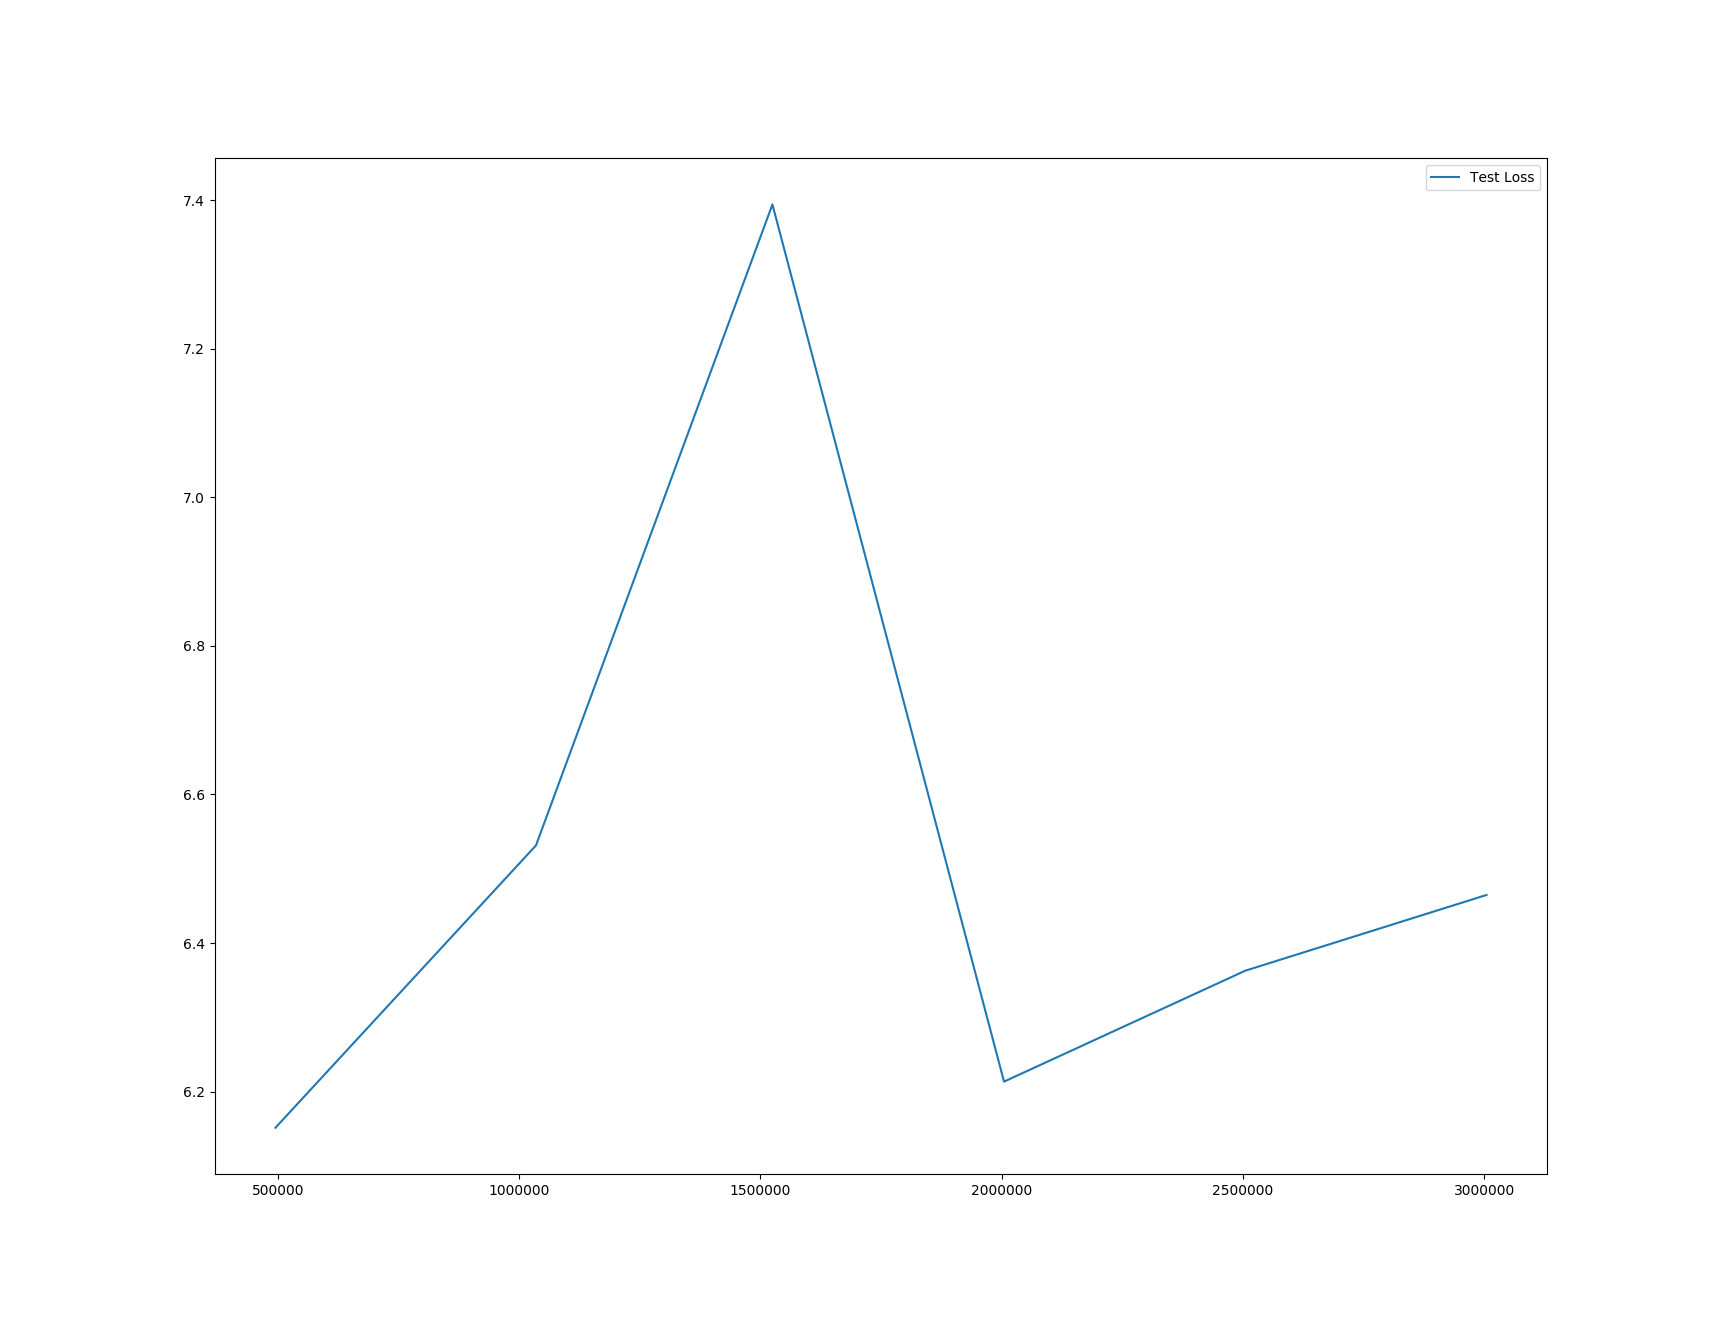
\includegraphics[width=\linewidth]{img/plots/opensubtitles_not_reversed/test_metrics_loss.png}
	\centering
	\small
	\text{Only the loss.}
	\endminipage\hfill
	\caption{The loss and perplexity by running the six different snapshots against the test dataset using the OpenSubtitles model.}
	\label{result:test_performance:opensubtitles}
\end{figure}

\begin{figure}[H]
	\minipage{0.5\textwidth}
	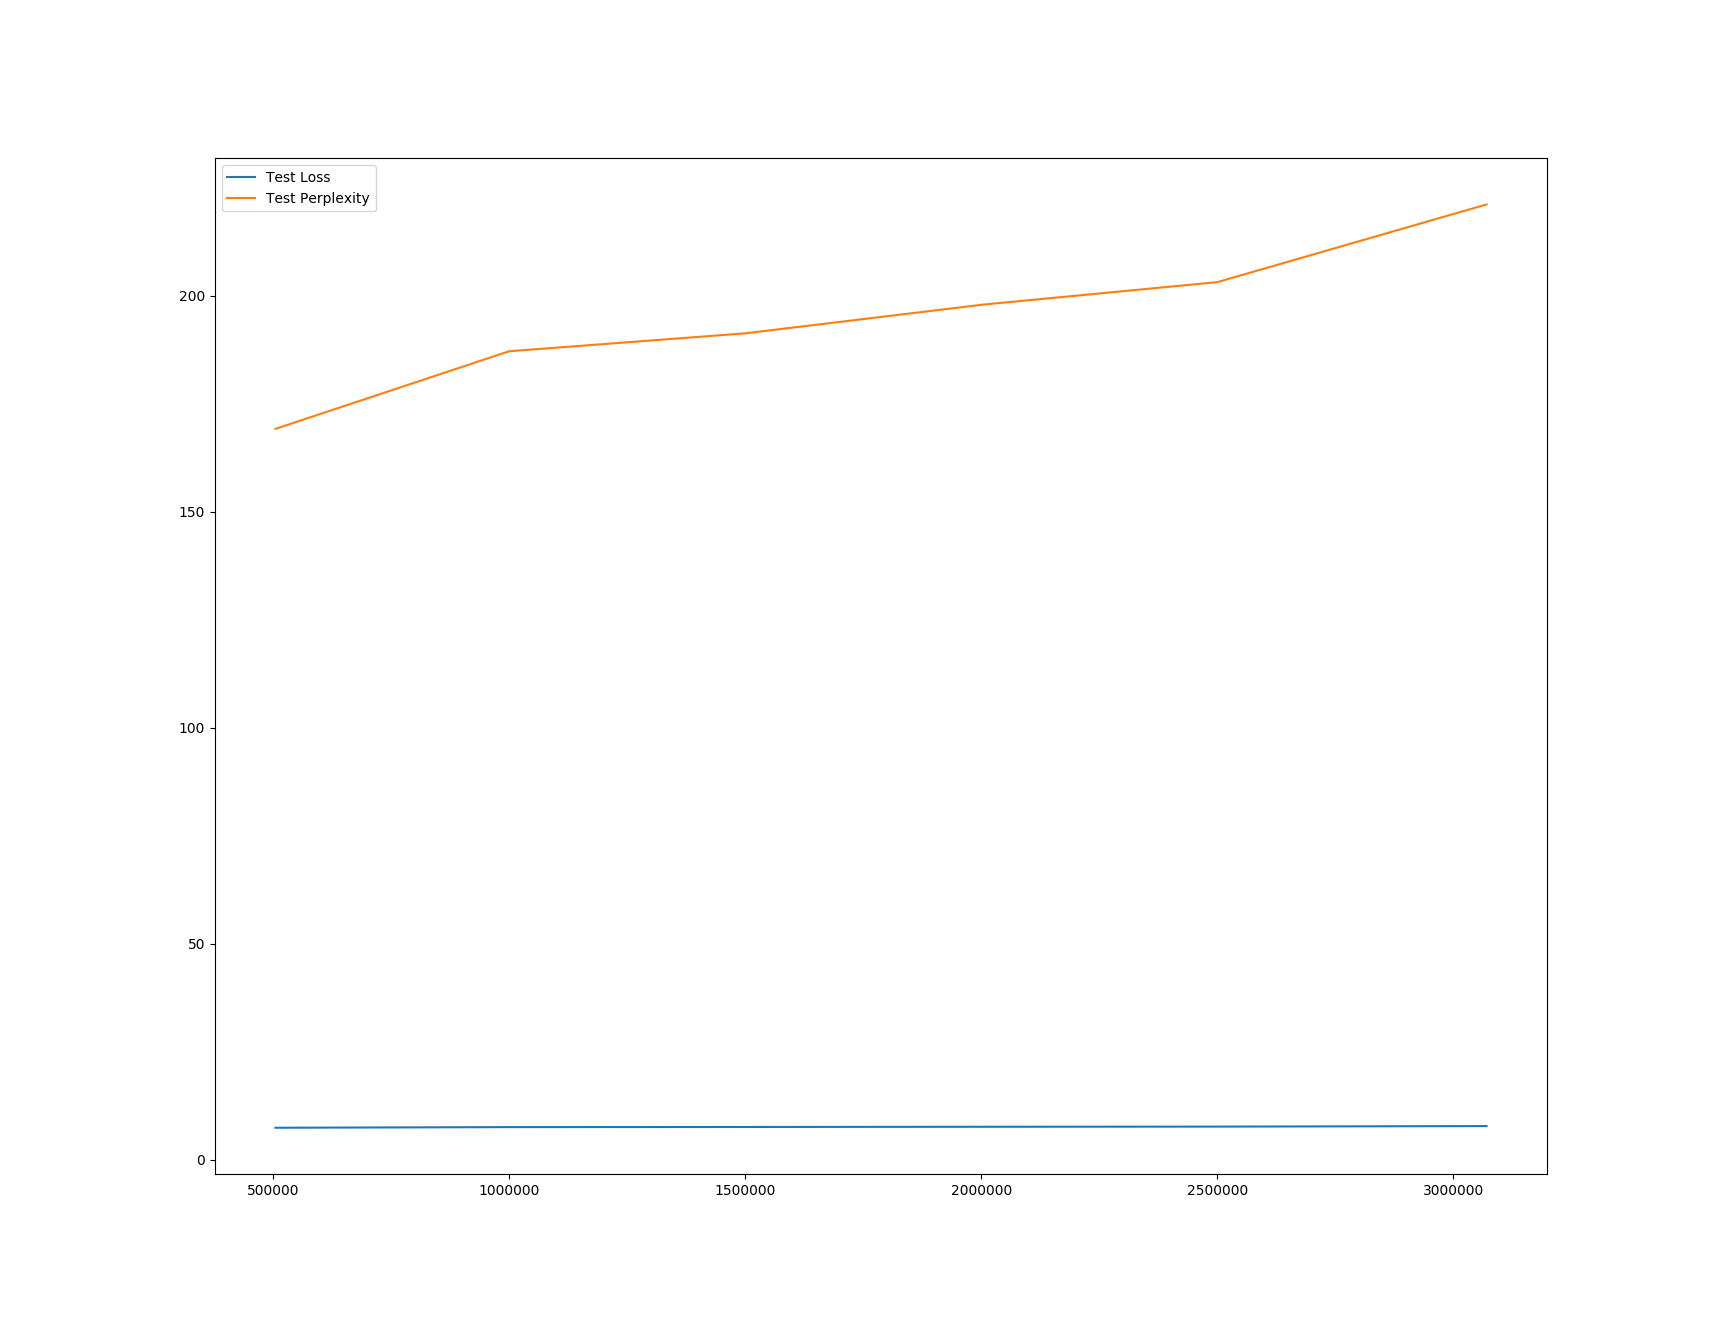
\includegraphics[width=\linewidth]{img/plots/reddit/test_metrics_both.png}
	\centering
	\small
	\text{The loss and perplexity.}
	\endminipage\hfill
	\minipage{0.5\textwidth}
	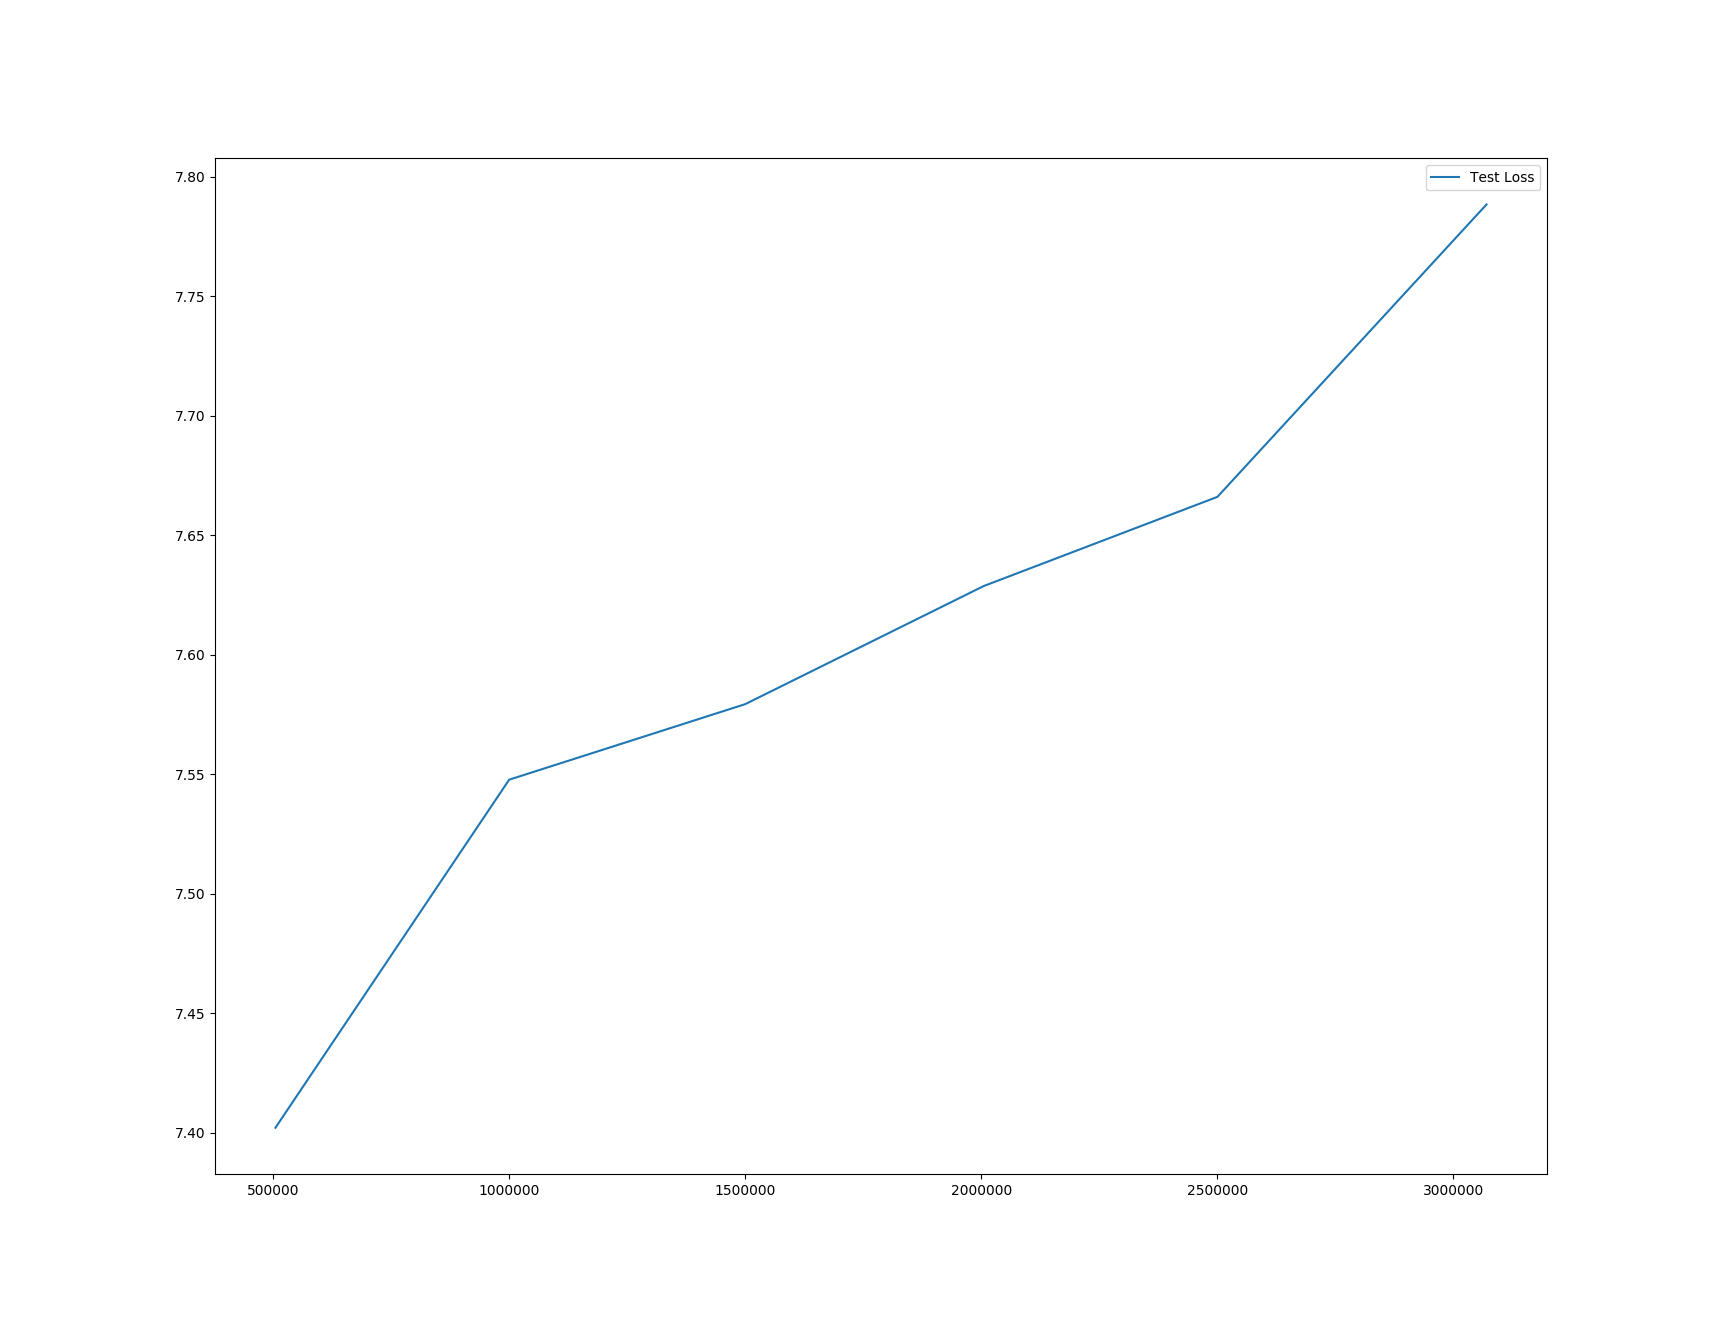
\includegraphics[width=\linewidth]{img/plots/reddit/test_metrics_loss.png}
	\centering
	\small
	\text{Only the loss.}
	\endminipage\hfill
	\caption{The loss and perplexity by running the six different snapshots against the test dataset using the Reddit model.}
	\label{result:test_performance:reddit}
\end{figure}

\section{Generated outputs over time}
\blindtext

\section{Comparison with CleverBot and ``Neural Conversational Model''}
\blindtext

\section{N-Gram Analysis}

\paragraph{OpenSubtitles} \blindtext
\begin{figure}[H]
	\minipage{0.5\textwidth}
	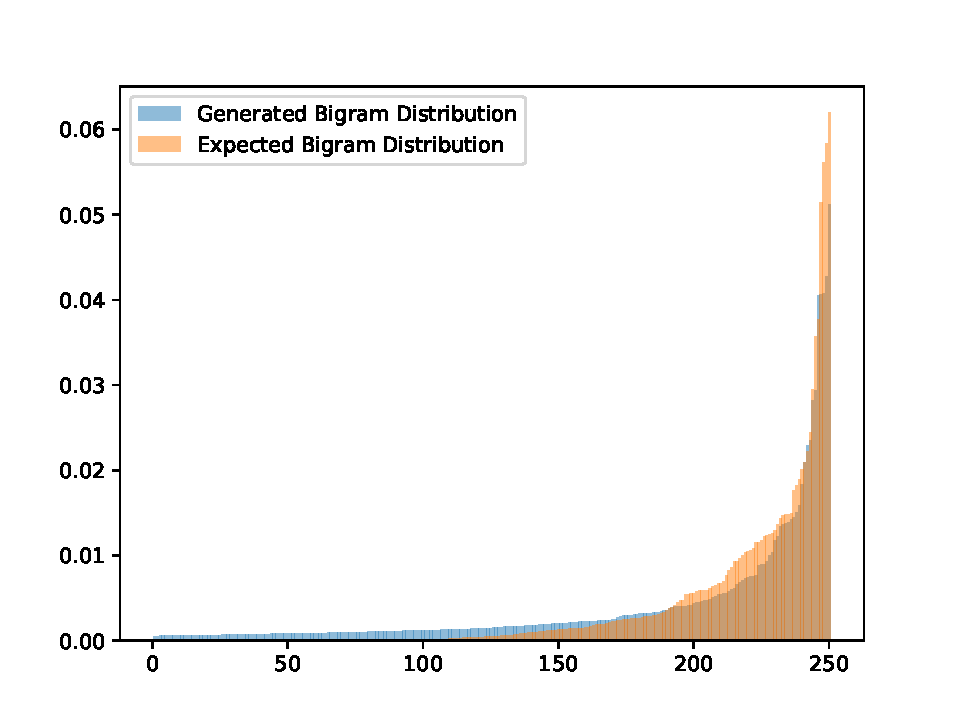
\includegraphics[width=\linewidth]{img/plots/opensubtitles_not_reversed/bigram_distribution_comparison_step_500000.pdf}
	\centering
	\small
	\text{Distribution at training step 500'000.}
	\endminipage\hfill
	\minipage{0.5\textwidth}
	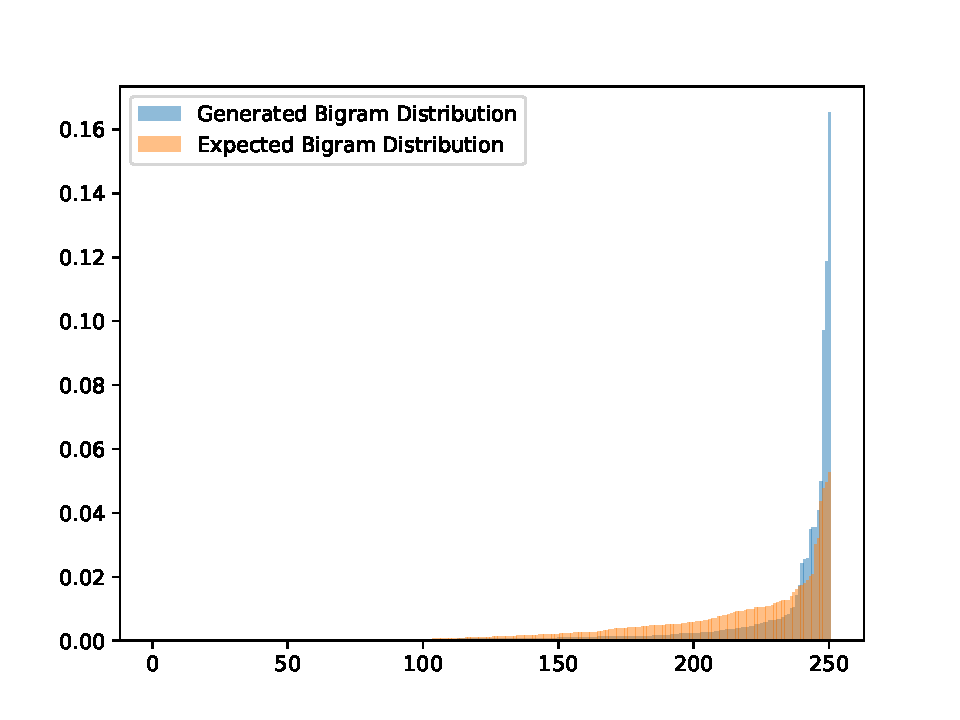
\includegraphics[width=\linewidth]{img/plots/opensubtitles_not_reversed/bigram_distribution_comparison_step_1000000.pdf}
	\centering
	\small
	\text{Distribution at training step 1'000'000.}
	\endminipage\hfill
	\minipage{0.5\textwidth}
	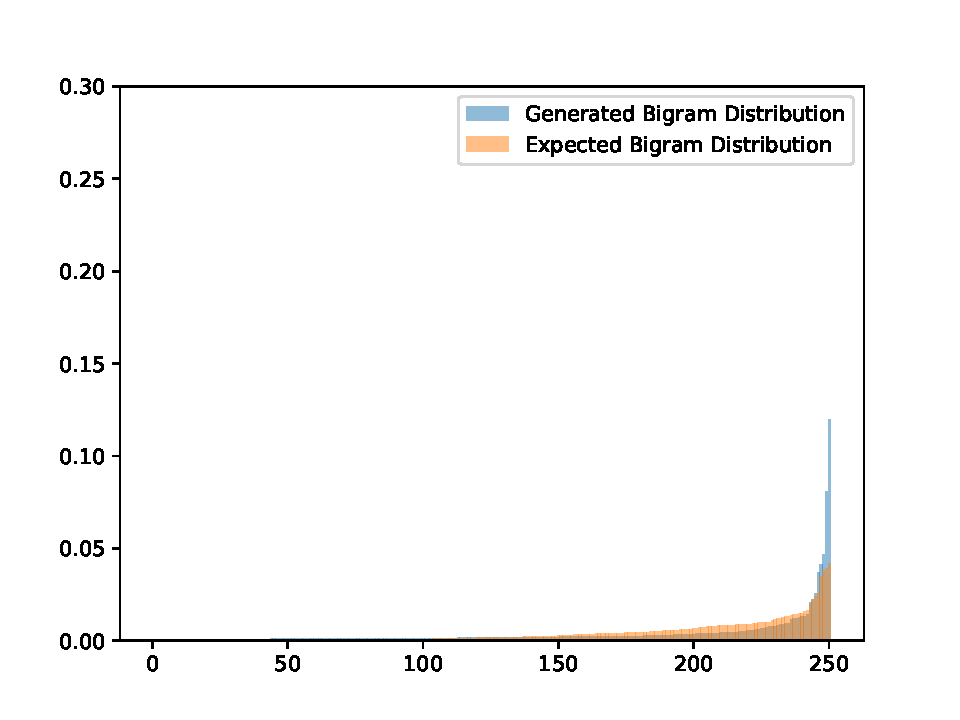
\includegraphics[width=\linewidth]{img/plots/opensubtitles_not_reversed/bigram_distribution_comparison_step_1500000.pdf}
	\centering
	\small
	\text{Distribution at training step 1'500'000.}
	\endminipage\hfill
	\minipage{0.5\textwidth}
	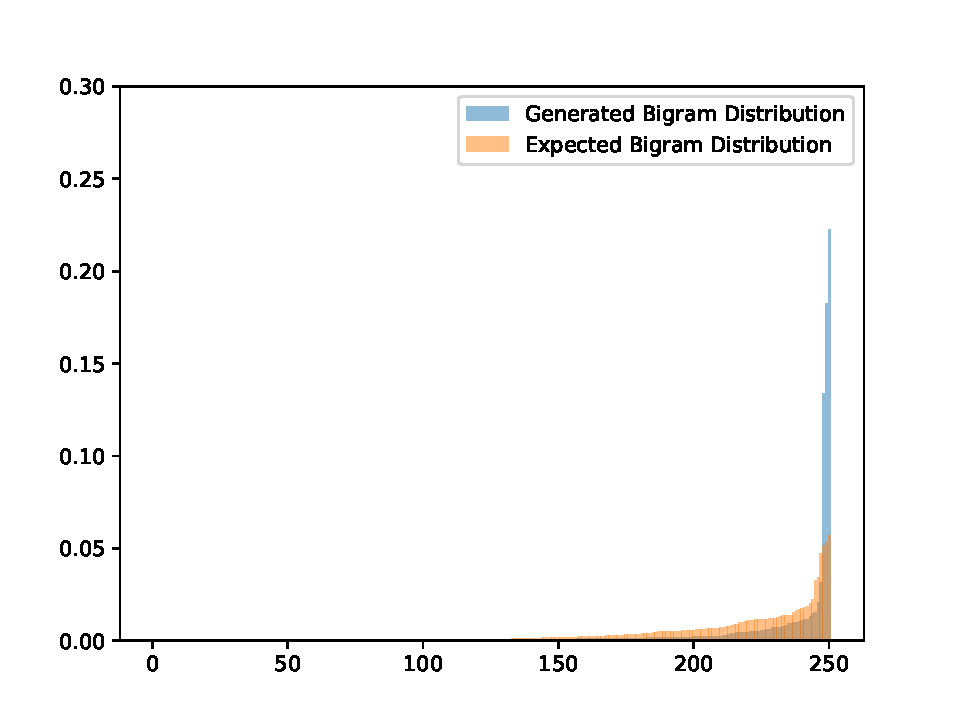
\includegraphics[width=\linewidth]{img/plots/opensubtitles_not_reversed/bigram_distribution_comparison_step_2000000.pdf}
	\centering
	\small
	\text{Distribution at training step 2'000'000.}
	\endminipage\hfill
	\minipage{0.5\textwidth}
	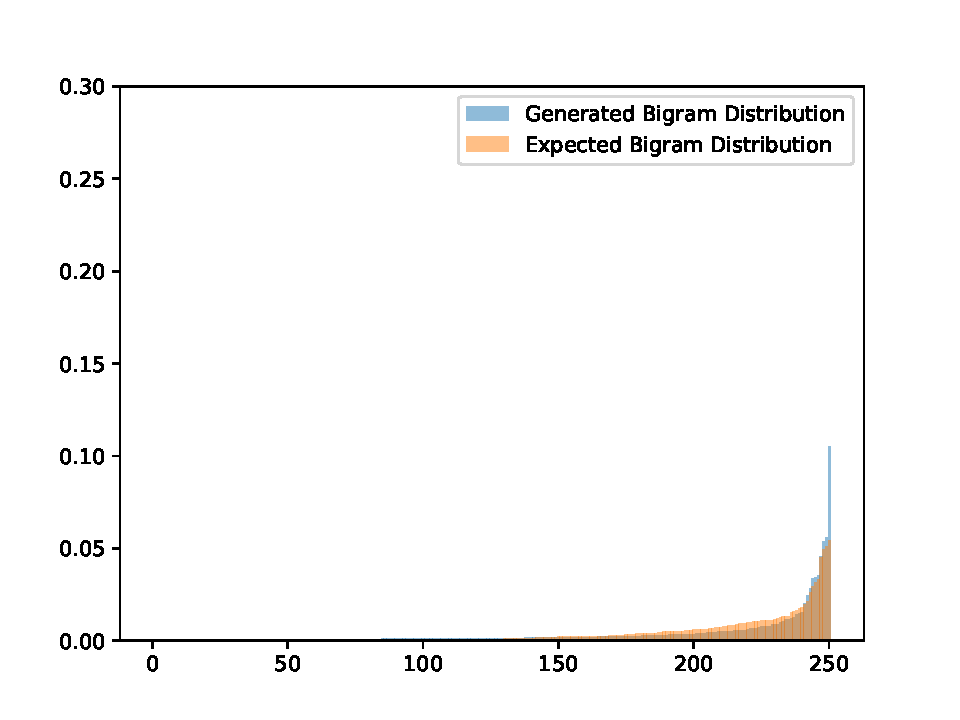
\includegraphics[width=\linewidth]{img/plots/opensubtitles_not_reversed/bigram_distribution_comparison_step_2500000.pdf}
	\centering
	\small
	\text{Distribution at training step 2'500'000.}
	\endminipage\hfill
	\minipage{0.5\textwidth}
	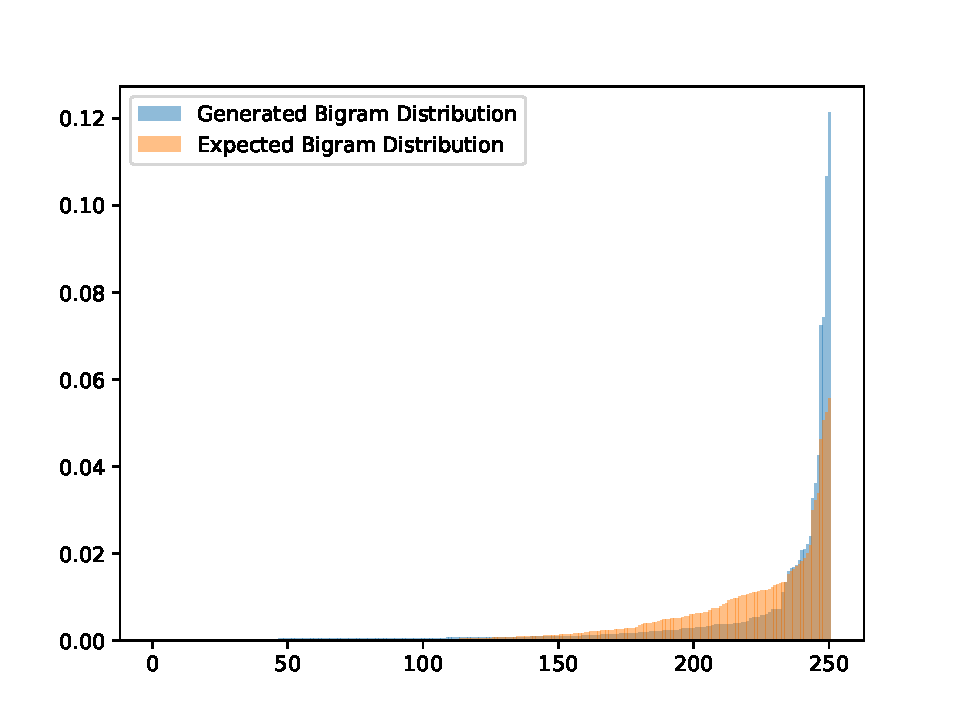
\includegraphics[width=\linewidth]{img/plots/opensubtitles_not_reversed/bigram_distribution_comparison_step_3000000.pdf}
	\centering
	\small
	\text{Distribution at training step 3'000'000.}
	\endminipage\hfill
	\caption{Distributions of the top 100 bigrams in the generated answers when using the test set over multiple time steps of the training.}
	\label{results:ngram:distributions:opensubtitles}
\end{figure}

\paragraph{Reddit} \blindtext
\begin{figure}[H]
	\minipage{0.5\textwidth}
	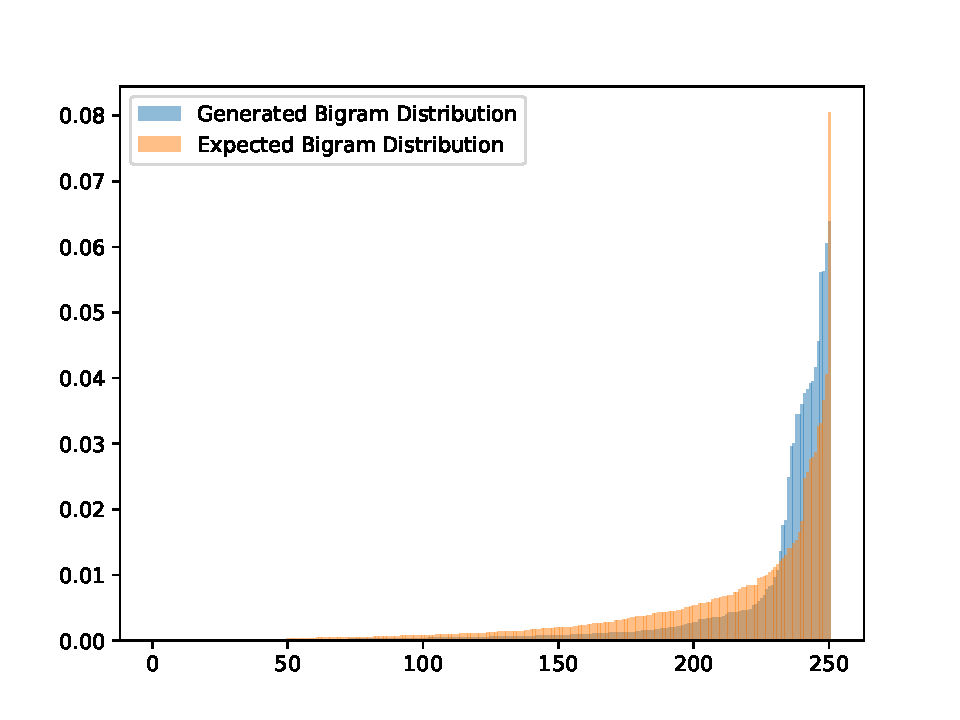
\includegraphics[width=\linewidth]{img/plots/reddit/bigram_distribution_comparison_step_500000.pdf}
	\centering
	\small
	\text{Distribution at training step 500'000.}
	\endminipage\hfill
	\minipage{0.5\textwidth}
	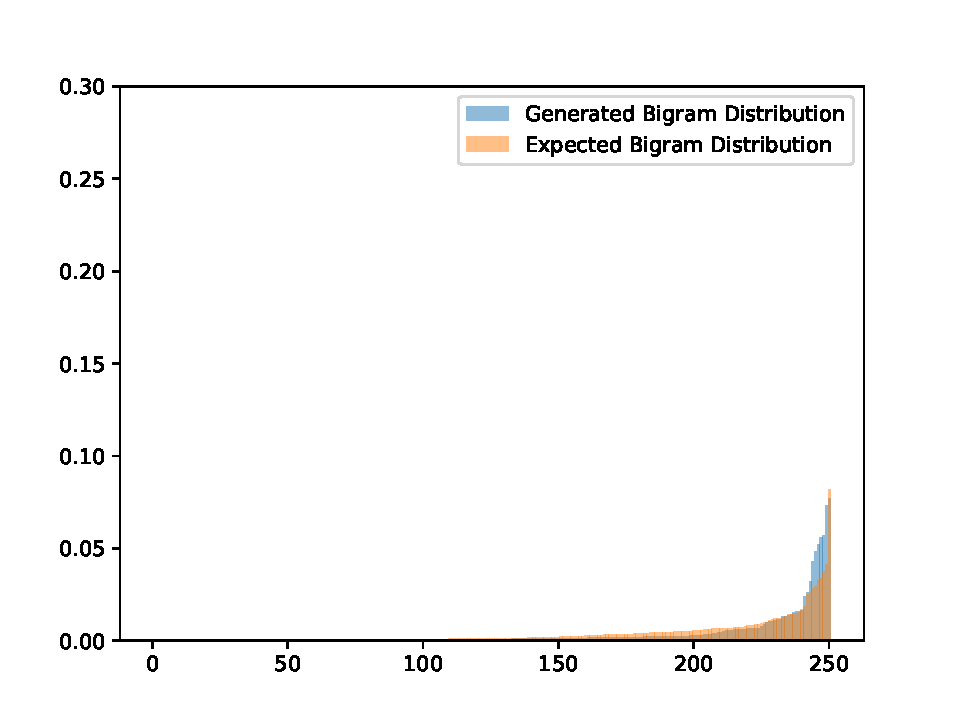
\includegraphics[width=\linewidth]{img/plots/reddit/bigram_distribution_comparison_step_1000000.pdf}
	\centering
	\small
	\text{Distribution at training step 1'000'000.}
	\endminipage\hfill
	\minipage{0.5\textwidth}
	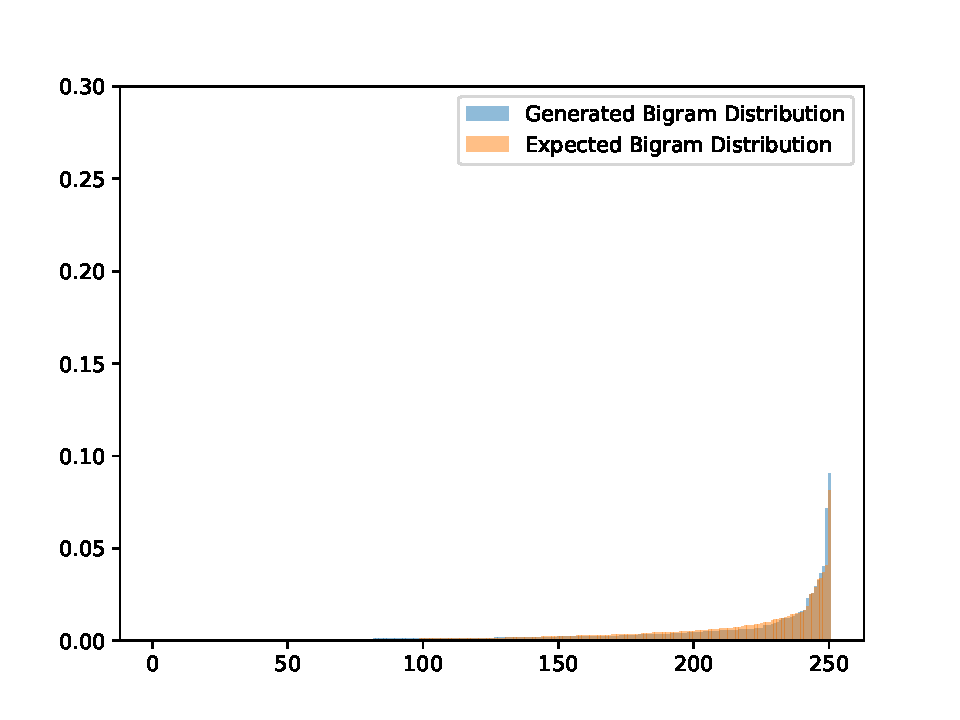
\includegraphics[width=\linewidth]{img/plots/reddit/bigram_distribution_comparison_step_1500000.pdf}
	\centering
	\small
	\text{Distribution at training step 1'500'000.}
	\endminipage\hfill
	\minipage{0.5\textwidth}
	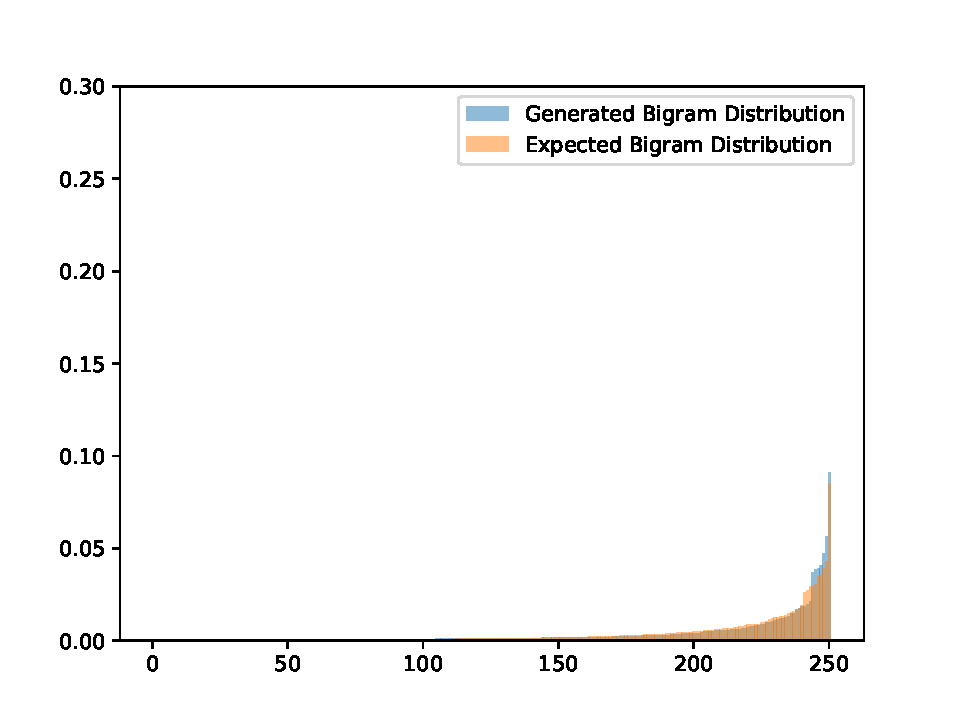
\includegraphics[width=\linewidth]{img/plots/reddit/bigram_distribution_comparison_step_2000000.pdf}
	\centering
	\small
	\text{Distribution at training step 2'000'000.}
	\endminipage\hfill
	\minipage{0.5\textwidth}
	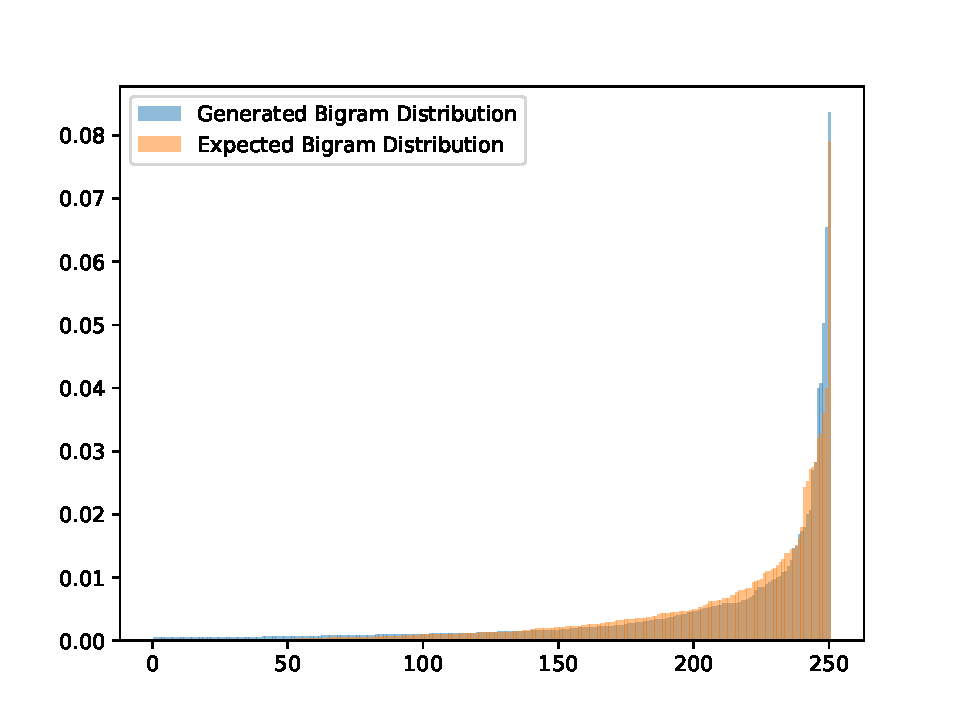
\includegraphics[width=\linewidth]{img/plots/reddit/bigram_distribution_comparison_step_2500000.pdf}
	\centering
	\small
	\text{Distribution at training step 2'500'000.}
	\endminipage\hfill
	\minipage{0.5\textwidth}
	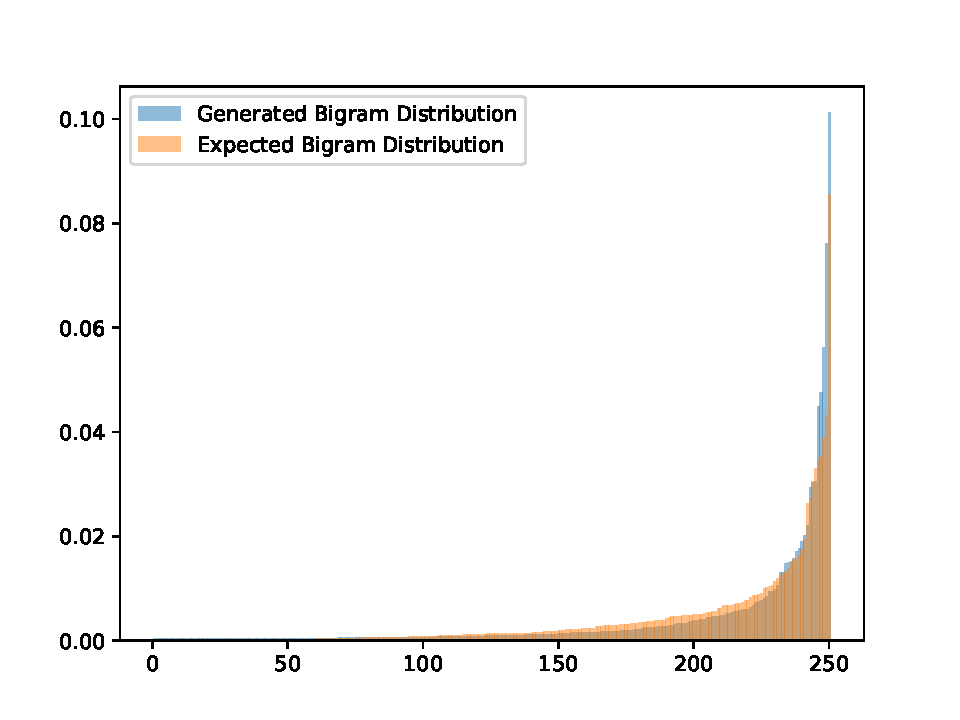
\includegraphics[width=\linewidth]{img/plots/reddit/bigram_distribution_comparison_step_3000000.pdf}
	\centering
	\small
	\text{Distribution at training step 3'000'000.}
	\endminipage\hfill
	\caption{Distributions of the top 100 bigrams in the generated answers when using the test set over multiple time steps of the training.}
	\label{results:ngram:distributions:opensubtitles}
\end{figure}

\section{Sent2Vec Analysis}
As described in Chapter~\ref{fundamentals:sent2vec_test}

\begin{figure}[H]
	\minipage{0.5\textwidth}
	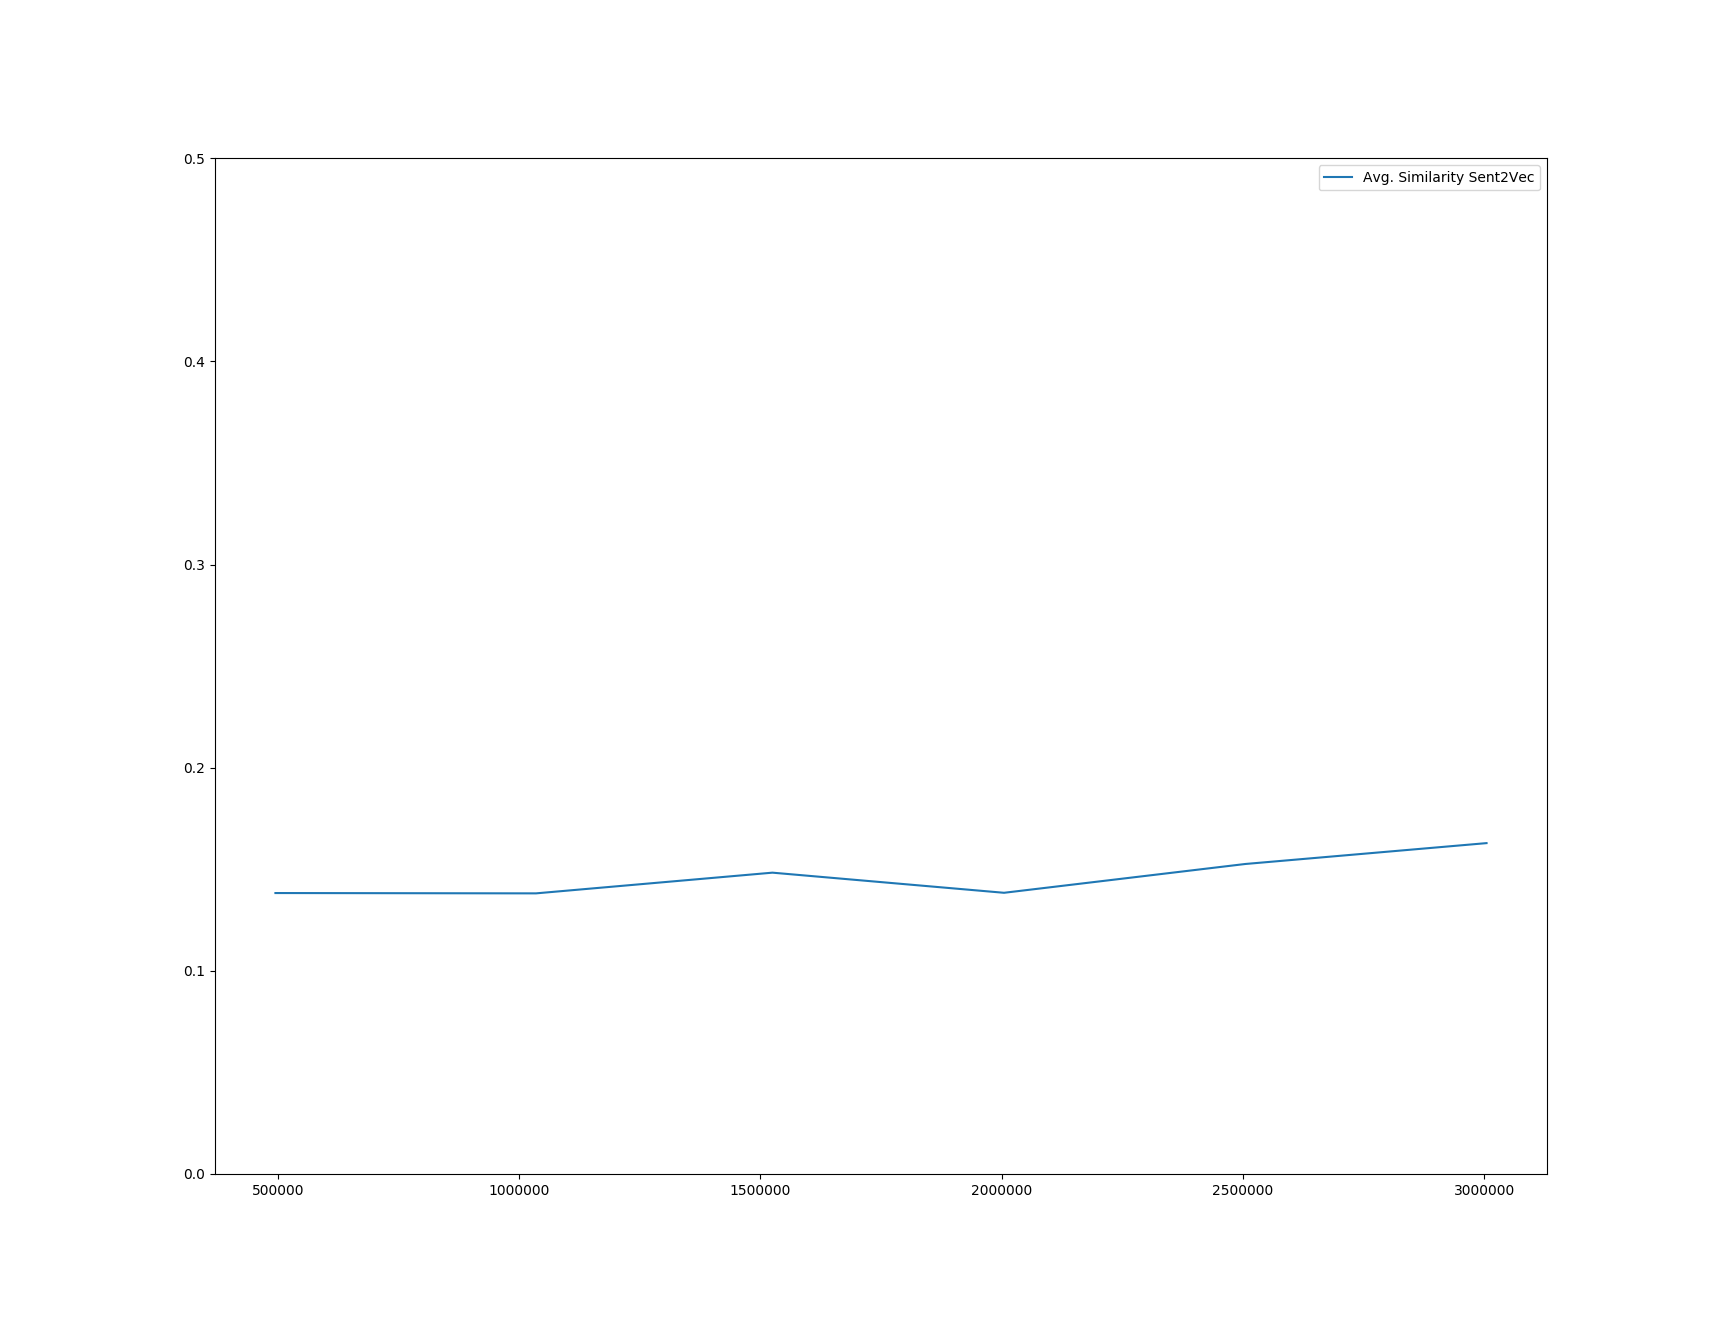
\includegraphics[width=\linewidth]{img/plots/opensubtitles_not_reversed/s2v_wiki_cosine_similarity.png}
	\centering
	\small
	\text{Evaluation with the wiki model.}
	\endminipage\hfill
	\minipage{0.5\textwidth}
	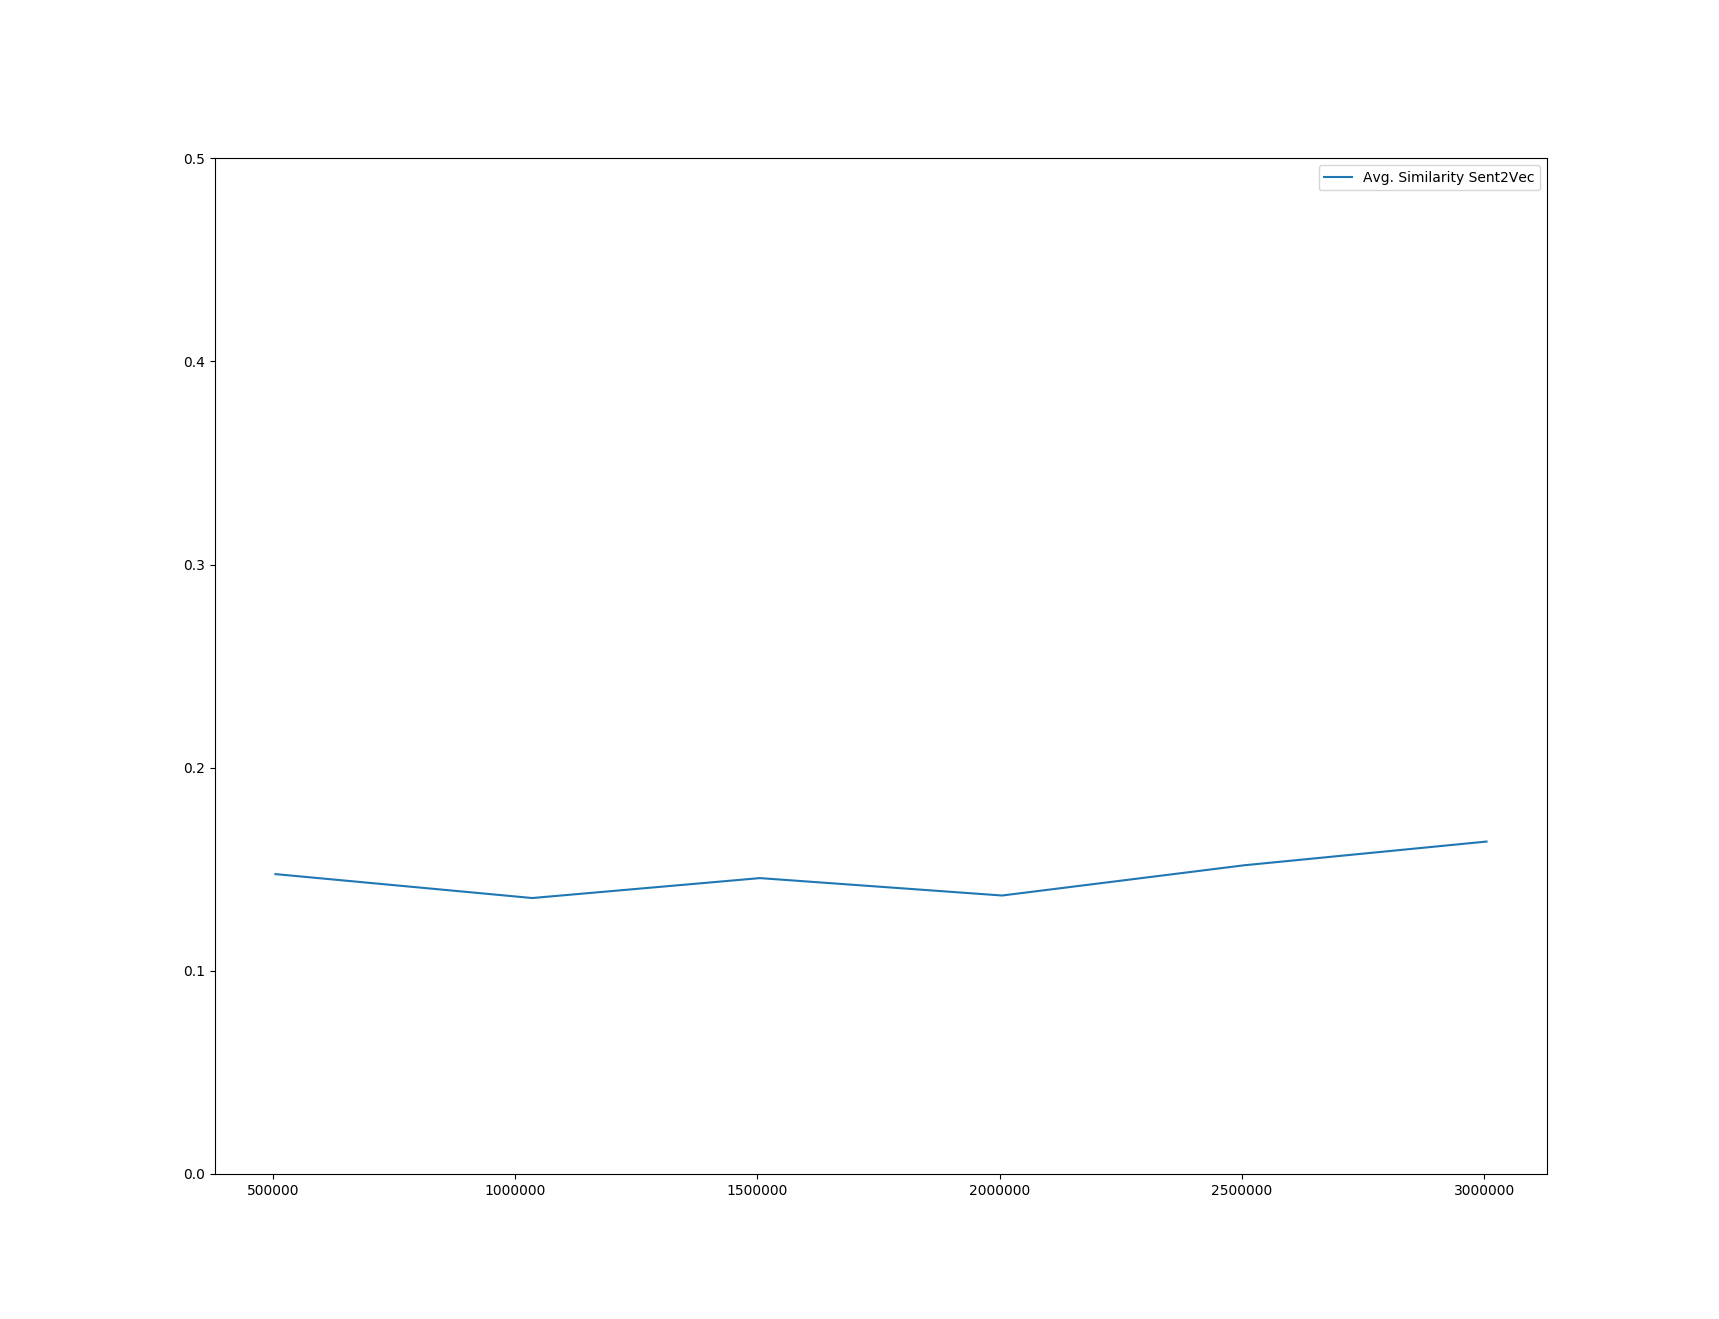
\includegraphics[width=\linewidth]{img/plots/opensubtitles_not_reversed/s2v_twitter_cosine_similarity.png}
	\centering
	\small
	\text{Evaluation with the twitter model.}
	\endminipage\hfill
	\caption{Results of the evaluation with Sent2Vec on the outputs of the OpenSubtitles models using the pretrained models found on the Sent2Vec GitHub page.}
	\label{results:sent2vec:opensubtitles:results}
\end{figure}

\begin{figure}[H]
	\minipage{0.5\textwidth}
	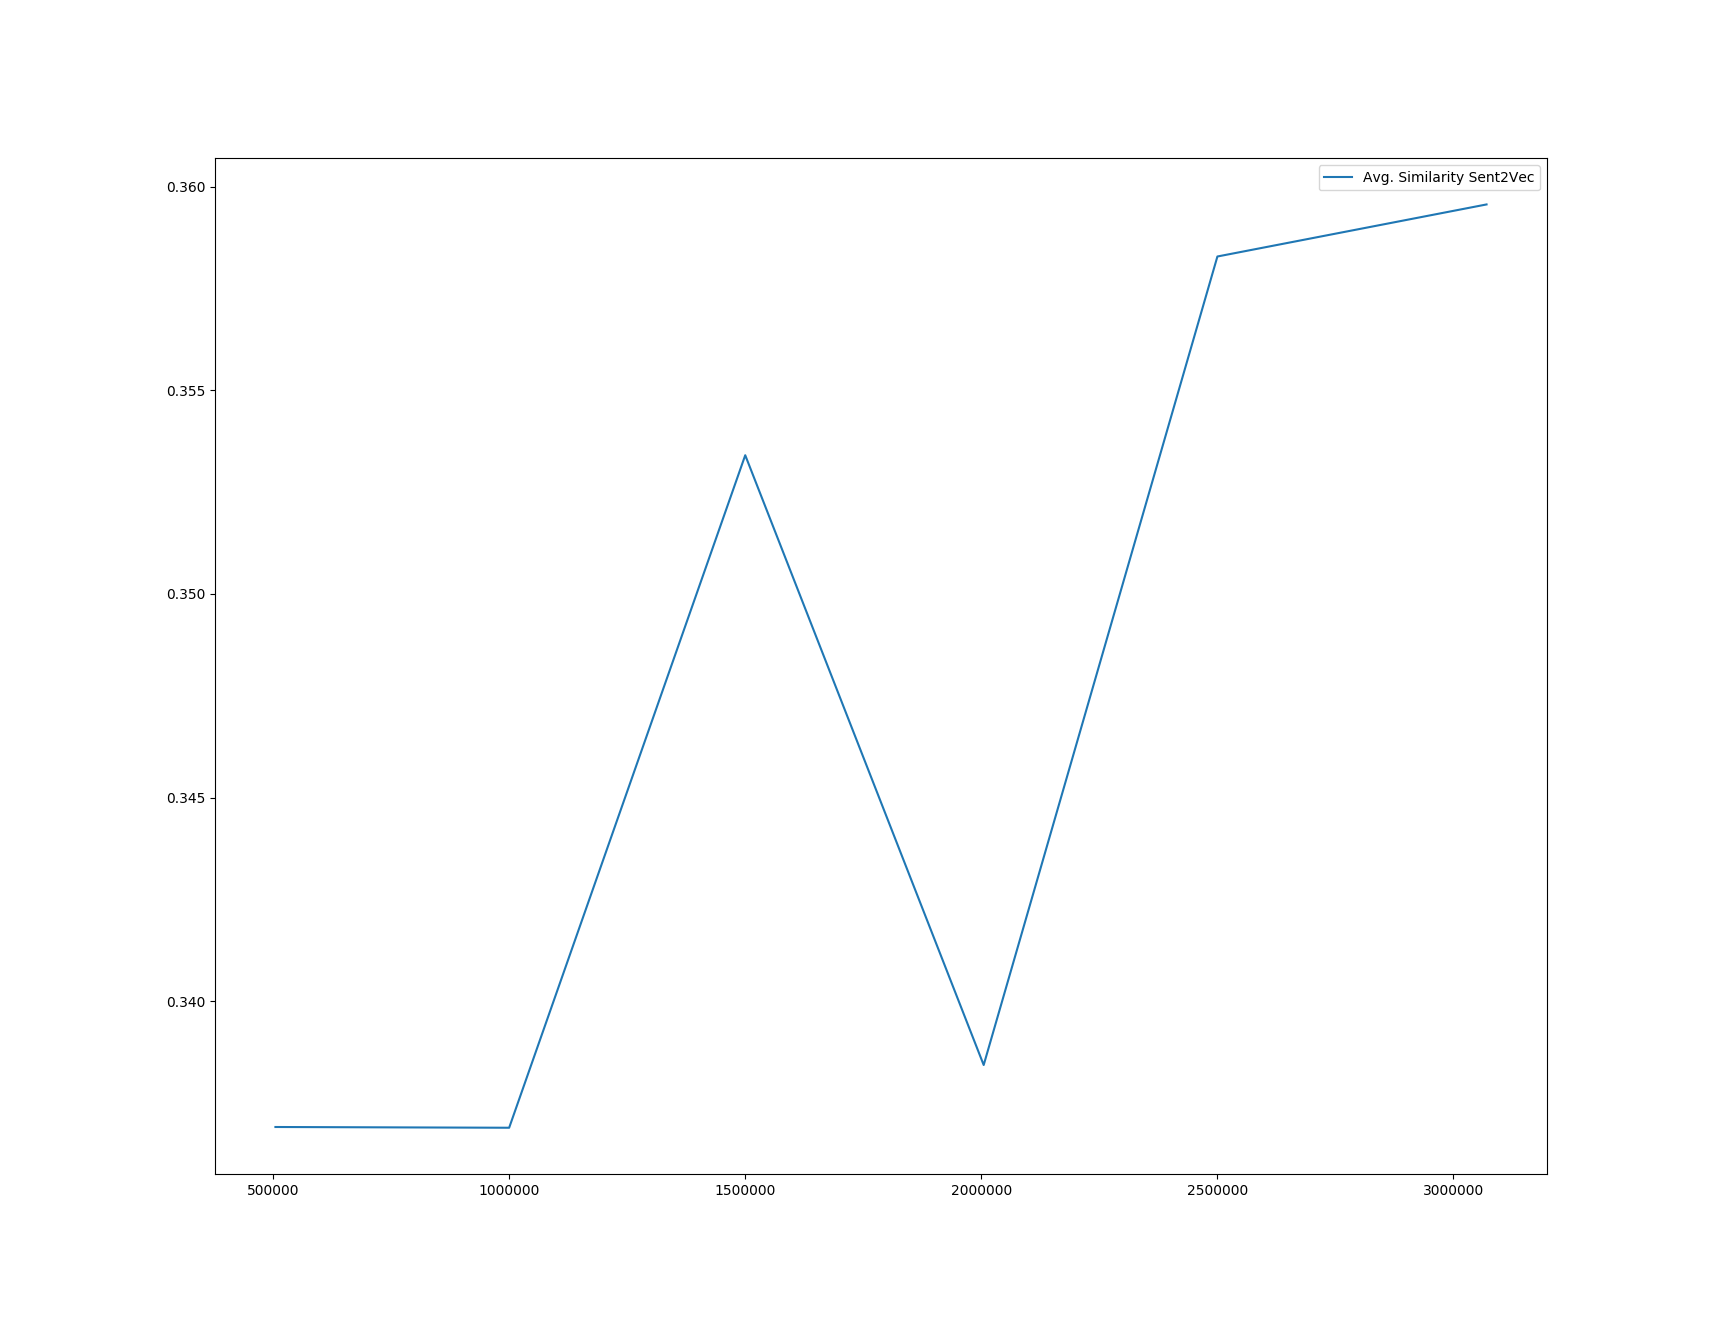
\includegraphics[width=\linewidth]{img/plots/reddit/s2v_wiki_cosine_similarity.png}
	\centering
	\small
	\text{Evaluation with the wiki model.}
	\endminipage\hfill
	\minipage{0.5\textwidth}
	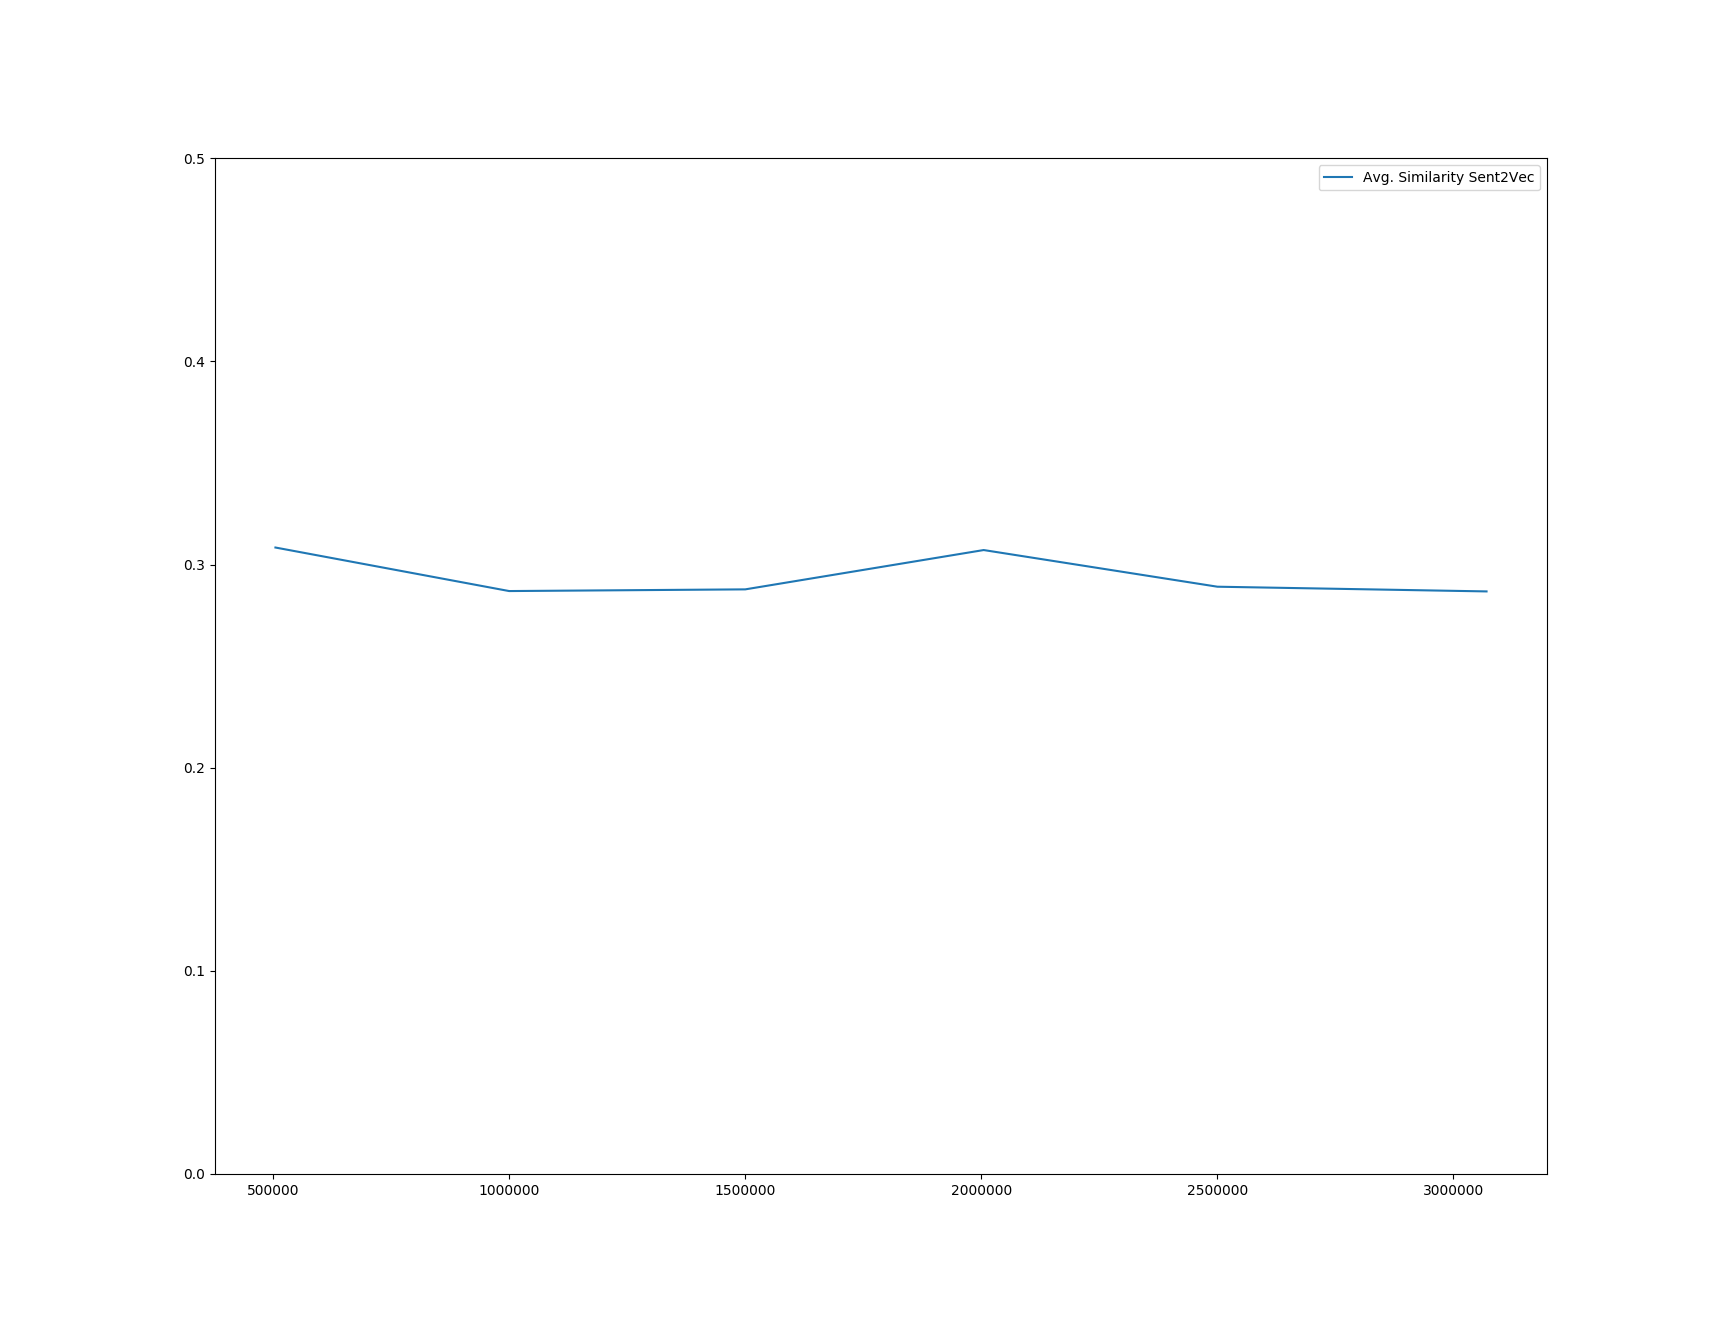
\includegraphics[width=\linewidth]{img/plots/reddit/s2v_twitter_cosine_similarity.png}
	\centering
	\small
	\text{Evaluation with the twitter model.}
	\endminipage\hfill
	\caption{Results of the evaluation with Sent2Vec on the outputs of the Reddit models using the pretrained models found on the Sent2Vec GitHub page.}
	\label{results:sent2vec:reddit:results}
\end{figure}
\footnotetext{https://github.com/epfml/sent2vec}

\section{Thought Vectors for Input Sequences}
After the encoder has processed the whole input sequences, it pass it forward to the decoder to construct the output sequence (see Chapter~\ref{fundamentals:seq2seq}). It is the only direct connection the encoder and decoder have in such a model, which means, that the encoder has to ``encode'' all the information into this thought vector before passing it to the decoder. The thought vector hence represents an embedding of the input sequence in an $n$ dimensional vector space, where $n$ stands for the size of the thought vector. To analyze this embeddings, we collected them for 15 different sample sentences and projected them via PCA into two dimensional space, the results of this projection can be see in Figure~\ref{results:thougth_vectors:embeddings:opensubtitles} and~\ref{results:thougth_vectors:embeddings:reddit} below.

\begin{figure}[H]
	\centering
	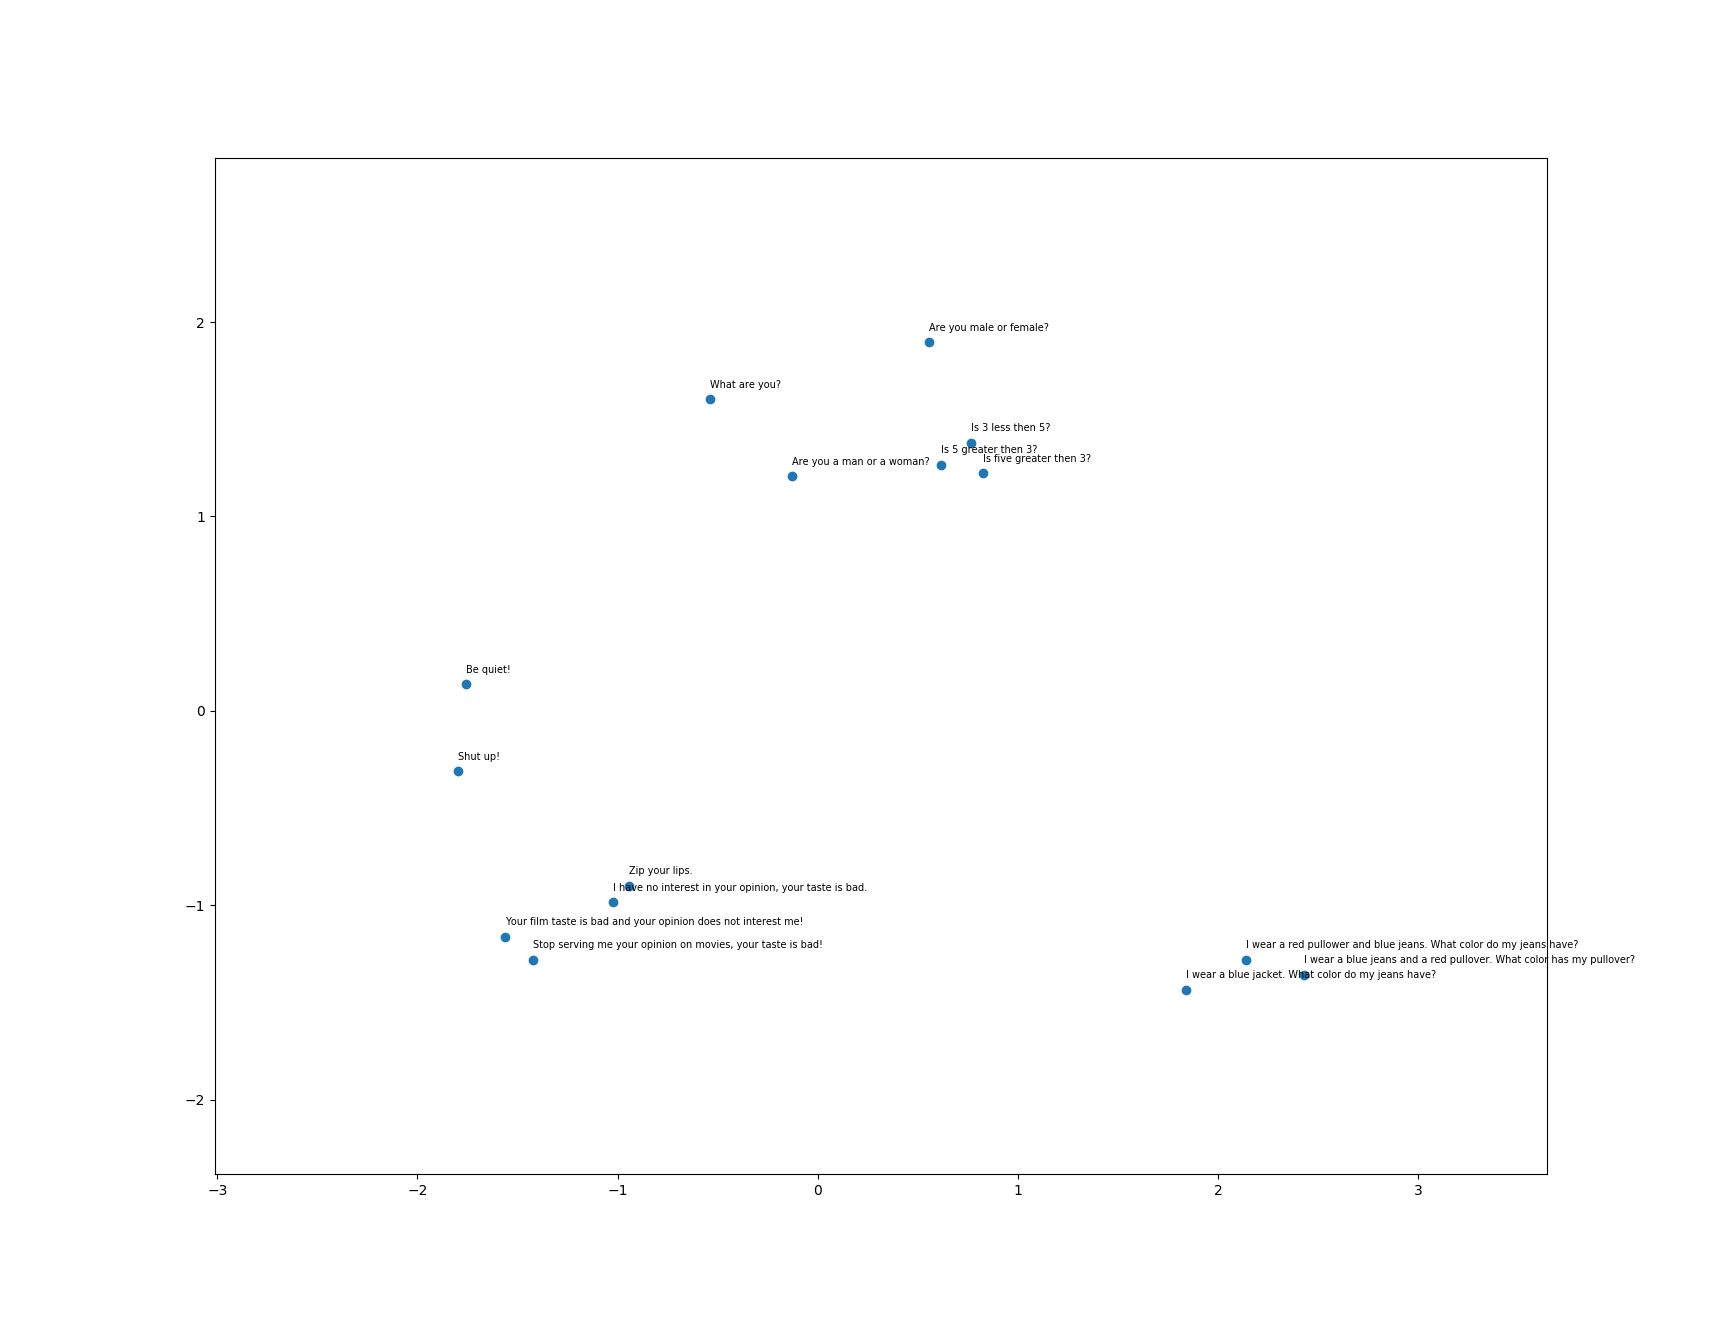
\includegraphics[width=16cm]{img/opensubtitles_thought_vector_embeddings.png}
	\caption{The projected thought vectors for 15 different sentences when using the OpenSubtitles model. PCA was used for the projection.}
	\label{results:thougth_vectors:embeddings:opensubtitles}
\end{figure}

\begin{figure}[H]
	\centering
	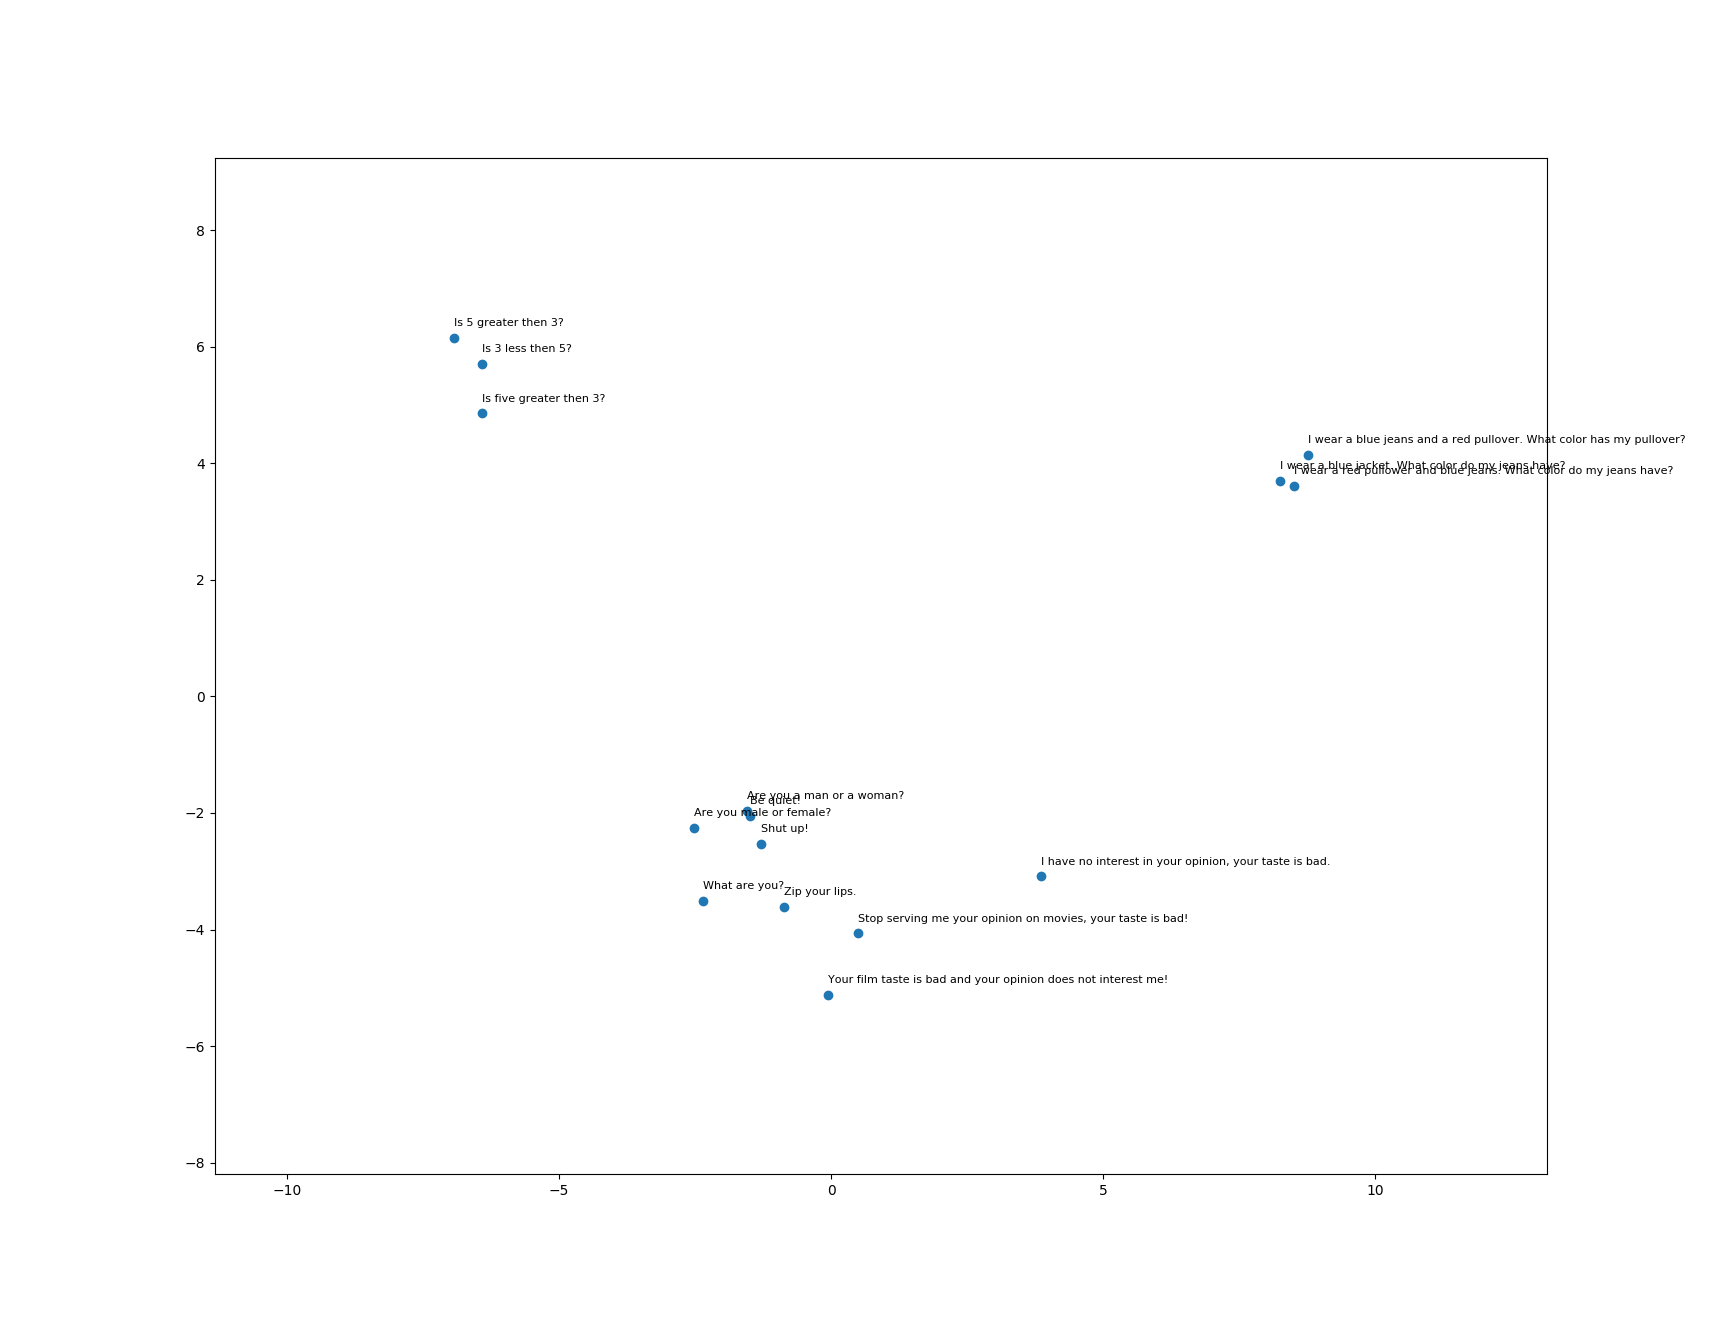
\includegraphics[width=16cm]{img/reddit_thought_vector_embeddings.png}
	\caption{The projected thought vectors for 15 different sentences when using the Reddit model. PCA was used for the projection.}
	\label{results:thougth_vectors:embeddings:reddit}
\end{figure}

Both of the models seem to have no problems understanding clear, direct sentences where the intent is clear (e.g. ``I have no interest in your opinion on movies, your taste is bad!''). This can be seen because similar sentences are clustered together in the projected space. However, when it comes to curses and questions regarding the gender, the OpenSubtitles model starts to struggle, which can be seen by taking a look at the respective points in the projected space. For example, the questions regarding the gender or the curses are scattered throughout the space, even though they should have been embedded closely to each other. The Reddit model seems to have less problems with this, as the embeddings for these sentences are quite close together. But what is interesting to see is that the Reddit model embeds the sentences with curses close to the sentences regarding the gender.\todo{write more}

\section{Reverse Input Feeding}
\blindtext